%&latex2e

\documentclass[twoside,draft]{article}
\usepackage{latexsym,e-journal}

\usepackage[letterpaper]{geometry}
\usepackage[utf8]{inputenc}
\usepackage[english]{babel}

\usepackage{amssymb,amsfonts,amsmath}

\usepackage[perpage,symbol*]{footmisc}
\usepackage[final]{graphicx}
\usepackage{pstricks}
\usepackage{cite}

\usepackage[varg]{txfonts}

\oddsidemargin=-0.20in
\evensidemargin=-0.20in
\topmargin=-30pt

\textwidth=498pt
\textheight=646pt


\begin{document}
%\begin{tableofcontents}
\begin{sloppypar}

\renewcommand{\refname}{References}
\renewcommand{\tablename}{\small Table}
\renewcommand{\figurename}{\small Fig.}
\renewcommand{\contentsname}{Contents}


\twocolumn[%
\begin{center}
\renewcommand{\baselinestretch}{0.93}
{\Large\bfseries BACK TO COSMOS

}\par
\renewcommand{\baselinestretch}{1.0}
\bigskip
F. M. Sanchez$^1\!$, \ V. A. Kotov$^2\!$, \ M. Grosmann$^3$, \ D. Weigel$^4$, \ R. Veysseyre$^5$, \ C. Bizouard$^6$, \ N. Flawisky$^7$, \ D. Gayral$^8$, \ L. Gueroult$^9$\\
{\footnotesize  $^1$ Pr. Universit\'{e} Paris 11, Orsay, France (retired).\rule{0pt}{12pt}
E-mail: hol137@yahoo.fr\\
$^2$Astronomer Crimean Astrophysical Observatory CrAO, Nauchny, Crimea, Russian Federation.
$^3$ Pr. at Universit\'{e} Louis Pasteur, Strasbourg, France (retired).
$^4$ Pr. at Universit\'{e} of Dijon and Paris 6, France (retired).
$^5$ Pr. at Ecole Centrale, Paris, France (retired).
$^6$Astronomer at OBSPM, Paris, France.
$^7$Architect / Math Instructor at Ecole Nationale Superieure d'Architecture, Paris Malaquais, France.
$^8$Computer Science Engineer.
$^9$Lecturer at Ecole Nationale Superieure d'Architecture Paris Malaquais, France (retired).

}\par
\medskip
{\small\parbox{11cm}{%
\hfill To the memory of Sir Michael Atiyah\\
The antique concept of permanent Cosmos is reintroduced as a perfect deterministic Computer, inverting the anthropic principle and interpreting the dimensionless parameters as optimal calculation bases. The later are unified in the Topological Axis, which exhibits the string theory dimension series 4k+2, with the emphasis on the values 26 (visible Universe) and 10 (the Hydrogen - Pion couple). The 1D extension of the Holographic Principle defines the Grandcosmos and a $10^{61}$ Trans-Plankian quantified time. This resolves at last the vacuum energy dilemma and confirms the matter-antimatter Oscillatory Bounce. The mathematics-physics fusion is proved by $10^{-9}$ precise relations, implying the Eddington's constant 137 together with the Atiyah's constant, showing Four Force Unification. The Holic Principle and Eddington's Theory must unlock Particle Physics,  with massive gluons and composite d quark. The standard evolutionary cosmology, based on the imperfect cosmological principle, will be excluded by the observation of mature galaxies in the very far-field, and the invariance of the CMB temperature.  

%Mature galaxies will be found in the far-field instead of a dark space, rejecting thus the evolutionary cosmology, ill-founded %o%%n the imperfect cosmological principle.

%% TODO: Insérer axe topologique
}}\smallskip
\end{center}]{%


\setcounter{section}{0}
\setcounter{equation}{0}
\setcounter{figure}{0}
\setcounter{table}{0}
\setcounter{page}{1}


\markboth{F.M. Sanchez,\ V.A. Kotov,\ M. Grosmann,\ D. Weigel,\ R. Veysseyre,\ C. Bizouard,\ N. Flawisky,\ D. Gayral,\ L. Gueroult, \textit{Back to Cosmos}}{\thepage}

Contents

1. The Principles of Hierarchy and Computation

2. The Cosmic Fine-Tuning and the Topological Axis

3. The Toponic Holographic Quantification

4. The Tachyonic Flickering Space-Time-Matter}

~~~   4.1. The Single Electron Cosmology
   
~~~    4.2. The Coherent Cosmic Oscillation (CCO)
   
~~~    4.3. The omnipresence of CCO in astrophysics
   
~~~    4.4. The Tifft, Arp and Pionner effects
   
5. The Logic of Dimensional Analysis

6. The Arithmetical Logic: Holic Principle

7. The Special Holographic Relations

~~~    7.1. The Conservation of Information
   
~~~    7.2. The Cosmic Temperature

~~     7.3. The Holic Principle and CCO 
    
8. The role of Intermediary Mathematical Constants

~~~    8.1. The Eddington's constant 137
   
~~~    8.2. The Atiyah and Sternheimer constants
   
~~~    8.3. The ubiquity of $a^a$
   
~~~    8.4. The intervention of Sporadic Groups
   
 9. The Fine-Tuning with basic mathematical constants
 
~~~    9.1. The optimal calculation base $e$ confirmed
   
~~~    9.2. The Lenz-Wyler's Formula
   
~~~    9.3. The Archimedes constant $\pi$ as a calculation base
   
~~~    9.4. The Four Force Unification in ppb Fine-Tuning
   
~~~    9.5. The Heavy Leptons Fine-Tuning
   
 10. Discussion
 
 11. Conclusions: Cosmic Simplicity at work
 
 12. Predictions
    
\markright{F.M. Sanchez,\ V.A. Kotov,\ M. Grosmann,\ D. Weigel,\ R. Veysseyre,\ C. Bizouard,\ N. Flawisky,\ D. Gayral,\ L. Gueroult, \textit{Back to Cosmos}}
\section{The Principles of Hierarchy and Computation}
\markright{F.M. Sanchez,\ V.A. Kotov,\ M. Grosmann,\ D. Weigel,\ R. Veysseyre,\ C. Bizouard,\ N. Flawisky,\ D. Gayral,\ L. Gueroult, \textit{Back to Cosmos}}

It was observed that the physical constants are tightly contrived, but only three dimensionless parameters: $a$, $p$, and $a_{G}$ are sufficient to explain the main structures of the world \cite{Carr}. Two of them are precisely measured: the electric constant $a$ $\approx$ 137.035999139(31), known with 0.23 ppb precision, and the proton-electron mass ratio $p$ $\approx$ 1836.15267245(75), known with 0.41 ppb precision. By contrast, the gravitational coupling constant $a_{G}$ was neither well defined nor measured, partially due to the relatively large imprecision on $G$ measurement 10$^{-4}\!$.

One can read \cite{Carr}: \textit{“For example, the size of a planet is the geometric mean of the size of the Universe and the size of an atom; the mass of man is the geometric mean of the mass of a planet and the mass of a proton. Such relationships, as well as the basic dependencies on $a$ and $a_G$ from which they derive, might be regarded as coincidences if one does not appreciate that they can be deduced from known physical theory, with the exception of the Universe, which cannot be explained directly from known physics... This line of arguments, which is discussed later, appeals to the 'anthropic principle'.”}

The existence of relations that are not explained by known physical theories, is called 'natural fine tuning' phenomena. But, as soon as it involves the observable Universe radius, it signals the existence of a more fundamental theory that must take into account the \textit{antique Cosmos concept, which, as Eddington claimed firstly \cite{Eddington}, must be permanent}. Extending this to the spatial homogeneity, this leads to the Perfect Cosmological Principle, the very foundation of the steady-state cosmology and the basis of Coherent Cosmology \cite{Sanchez1}.

So Eddington considered rightly the Cosmic Large Number correlations, as recalled in this article. However, his work was rejected for obscure reasons and this rejection was enforced by the fact that about 30 dimensionless parameters appear as 'free parameters' in the Particle standard model. They are misnamed since far from being really 'free', they are imposed by Nature. Nevertheless, a large majority of theorists believe they are due to chance, leading to a separation between Physics and Mathematics, not to speak of Biology. Thus, through the above Anthropic Principle, a majority believe in the Multiverse conundrum, a multiplicity of sterile Universe \cite{Carr}.

The present article shows that \textit{Physics is a unique part of Mathematics, which are presently incomplete}, refuting the Multiverse Hypothesis by very precise fine-tuning ($10^{-9})$ between main physical and mathematical constants: $\pi$, $e$ and $\gamma$, the Euler-Mascheroni constant. Also, this study confirms the super-string theory, but with complete rehabilitation of the \textit{tachyonic} bosonic string theory.

\textit{A decisive point of physics is the energy conservation, the First Principle of Thermodynamics.} Theorists associate it with time uniformity, but a more direct and logical explanation is that cosmos is a computer, so Intelligent Life receives a justification: to help the Cosmos computation. This Inverted Anthropic Principle answers the first of all questions: why one asks questions? We propose that the parameters are optimal base in a Deterministic Computing Cosmos, and they appear indeed in DNA characteristics and triple-point temperatures of mammals and main molecules \cite{Sanchez1}.

\textit{This reinstates the Laplace determinism}, involving non-local hidden variables, which are identified with the Cosmos, so rejecting the standard Copenhagen statistical interpretation of quantum mechanics.

The fact that three parameters, among 30, are so clearly emerging means that physics, and more generally science, follows a hierarchical order: \textit{one can progress without knowing the details of the underlying fundamental theory.}

So, when Proust and Dalton found whole numbers in chemical reactions, they were prefiguring atomic physics. The same for Balmer, spectral lines and wave mechanics. Idem for Mandeleiev, atomic masses and nuclear physics. Also, when Mandel found whole numbers in Biology, he anticipated genetics. 

In the same manner, this article prefigures \textit{the fundamental theory, but precising its arithmetical foundation: the Holic Principle}, recalled in section 6. Thus, there must exist multi-base algorithms able to explain the compatibility between these two principles, which seems at first sight contradictory. 


\begin{figure*}
\centering
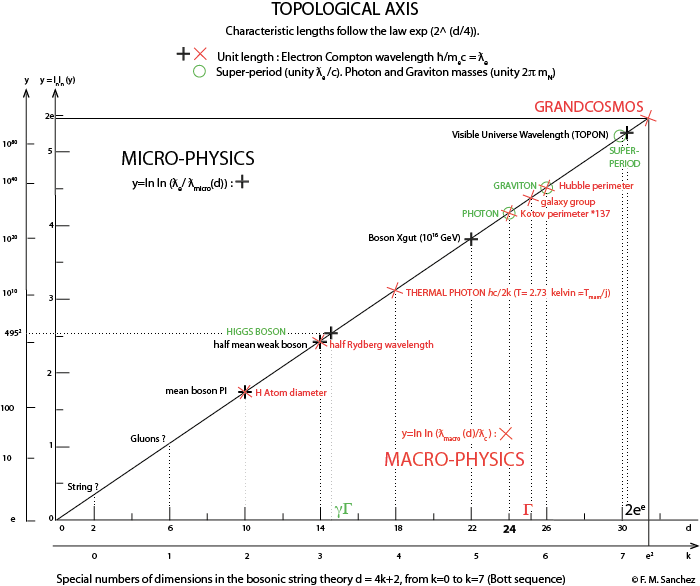
\includegraphics[width=\textwidth,height=14cm]{./figures/figure}
\caption{The Topological Axis. Double natural logarithms (y = lnln(Y)) of main dimensionless physical quantities 
(Y) corresponds to the String dimension series n = 4k + 2, from k = 0 to k = 7, showing the Bott
periodicity 8 [19] which is at the origin of the name `Topological Axis`. 
\textit{With unit the Electron Compton wavelength, in the macro-physics side}, the Universe circumference 
    is tied to the bosonic critical dimension 26, while Bott reduction leads to n = 18 (thermal photon, 
    tied to the the mammal wavelength through the Sternheimer scale factor j), n = 10, (super-string 
    dimension, Hydrogen atom), and n = 2 (string). For the number 24 of transverse dimensions, it is
    the Kotov length, through a factor 2$\pi a$, with $a \approx 137.036$. For $n \approx \Gamma $, the Atiyah constant, it means the galaxy group radius, a characteristic cosmic length ($10^{6}$ ligth-years). For $k \approx e^{2}$, $y \approx 2e$, it is the Grandcosmos radius.
   \textit{With the same unit, the Electron Compton wavelength, in the micro-physics side}, the Space-Time-Matter
    Holic dimension n = 30 is tied to $c$ times the cosmic Supercycle period, while Bott reductions lead to the gauge bosons:
    n = 22 (GUT bosons, $10^{16} GeV$), n = 14 (weak bosons) and n = 6 (massive gluons, about 10 MeV).
    For the superstring n = 10, it is the Pion. For $k \approx \pi$, n $\approx \gamma \times \Gamma$, Y $\approx 496^2$ 
    the square of the Green-Schwarz string dimension and the tenth root of the Monster cardinal, it is
    the Brout-Englert-Higgs boson (125 GeV). For k $\approx 2e^e$, it is the Topon, the visible Universe wavelength,
    which identifies with the mono-radial unit length of the Bekenstein-Hawking Universe entropy.
   \textit{With unit the electron mass}, n = 24 would correspond to the photon mass, while n $\approx \Gamma$, 
    to the graviton mass.
    \textit{With unit the Kotov length}, the Holic dimension n = 30 corresponds to the Monster cardinal, 
    apart a $\sqrt2$ factor.}
    The central dimension is n = 16, suggesting that the whole schema is tied to the Eddington's matrix $16 \times 16$.
\label{fig:figure_label}
\end{figure*}


\markright{F.M. Sanchez,\ V.A. Kotov,\ M. Grosmann,\ D. Weigel,\ R. Veysseyre,\ C. Bizouard,\ N. Flawisky,\ D. Gayral,\ L. Gueroult, \textit{Back to Cosmos}}
\section {The Cosmic Fine-Tuning and the Topological Axis}
\markright{F.M. Sanchez,\ V.A. Kotov,\ M. Grosmann,\ D. Weigel,\ R. Veysseyre,\ C. Bizouard,\ N. Flawisky,\ D. Gayral,\ L. Gueroult, \textit{Back to Cosmos}}

We look here for a systematic organization of dimensionless physical quantities stemming from cosmology, astrophysics, particle   physics, theoretical physics and mathematics. The most famous fine tuning implies cosmic quantities, awkwardly called the `Double Large Number Problem`. If it is a `problem` for standard evolutionary cosmology, it is a precious clue in the steady-state cosmology based on the \textit{Perfect} Cosmological Principle (spatial \textit{and} temporal homogeneity).
This Cosmological Fine-Tuning leads directly to a \textit{Gravitational Hydrogen molecule model of the visible universe} \cite{Sanchez1}.
Defining the Universe horizon radius with $R = 2a_{G} \lambdabar_{e}$, where the factor 2 comes from the bi-atomic structure, where $\lambdabar_{e} = \hbar/cm_{e}$ is the Electron Compton reduced wavelength, and the gravitational coupling constant is: 
$a_{G} = \hbar c/Gm_{p}m_{H}$, where $m_p$ and $m_H$ are the proton and hydrogen atom masses. So, \textit{the speed $c$ is eliminated}, in accordance with Coherent Cosmology which needs signal celerity far exceeding $c$. This gives $R \approx 13,812~Gly $, corresponding to a Hubble constant 70.790 (km/s)/Megaparsec, compatible with the most recent measurements \cite{Bonvin}: 72(3) (km/s)/Megaparsec. The latter confirms the value measured by the 1a type novae, while the standard optimization of 6 parameters results in a lower value, by $9\%$.

Consider the wavelength of the visible Universe with critical mass $M= Rc^2/2G$: $$\lambdabar_{M} = \hbar /Mc \approx 4 \times 10^{-96} m$$ This `Topon` is close to the touchstone n = 30 of the Topological Axis, see Fig. 1. The Topological Axis illustrates the function $f(n + 4) = f^{2}(n)$
and stems from the imbrication of relations of the form $\lambdabar_{e} /l_{micro} \sim (l_{macro} /\lambdabar_{e})^{2}$, followed by $ l_{macro} /\lambdabar_{e} \sim (\lambdabar_{e} /l^{\prime}_{micro} )^{2}$, leading to:
$$
\begin{array}{ll}
%
\displaystyle
\lambdabar_{e}/\lambdabar_{M} \sim (R/\lambdabar_{e})^{2} \sim (\lambdabar_{e}/ \lambdabar_{X})^{4}\\[+8pt]  % 1st row
\sim (\lambda_{CMB}/ \lambdabar_{e})^{8} \sim (\lambdabar_{e}/\lambdabar_{W})^{16} \sim (2r_{H} /\lambdabar_{e})^{32}\\[+8pt] % 2nd row
\sim (\lambdabar_{e}/ l_{Gl} )^{64} \sim (\lambdabar_{str} /\lambdabar_{e} )^{128} \sim 2^{256}\\ % 3rd row
\end{array}
$$
These series include the Cosmic Microwave Background wavelength $\lambda_{CMB}$ and a string wavelength $\lambdabar_{str}$, with mass about 2 MeV. Hence, the correlation is eight-fold, including, apart from the two above relationships, three relations that have been independently reported \cite{Sanchez1}. The overall large number $2^{256}$ has an obvious computational characteristic, confirmed below by the dramatic appearance of the Eddington Large Number.

In particular, the relation $R/\lambdabar_{e} \sim (\lambda_{CMB} / \lambdabar_{e})^{4}$ ties two cosmic lengths, the Hubble radius and the CMB wavelength by a relation that is incompatible with the standard evolutionary cosmology. By this order of magnitude, we infer rather precise relations. With the Hydrogen radius $r_H$, we infer 
$ R/r_H \approx (4\pi \lambda_{CMB}/r_H)^{4}$, precise to $0.6\%$. 
Considering the standard cosmological neutrino background (CNB), which wavelength is defined by $(\lambda_{CNB} / \lambda_{CMB})^{3} = 11/4$, we note that $R/ \lambdabar_{e} \approx
( \lambda_{CNB}^{2} / \lambda_{CMB} \lambdabar_{e} )^{4}$ to $1.7\%$. The appearance of the neutrino field is conform with the synthesis of the two main cosmologies, where the single Bang is replaced by a matter-antimatter Oscillatory Bounce \cite{Sanchez2}.

It was noted in \cite{Carr} that $a_{G}$ is of order $W^{8}$, where $W$ is the mass ratio W boson-Electron. With the above $R$ value, one observes the following more symmetrical relation involving the other (neutral) weak boson Z, in the 0.01\% indetermination of $W$ and $Z$:
\begin{equation}
R/(\lambdabar_{p}\lambdabar_{H})^{1/2}\approx (WZ)^4
\end{equation}
where $\lambdabar_{p}$ and $\lambdabar_{H}$ are the Proton and Hydrogen reduced wavelengths. The precision of this formula will be pulled to the ppb range in section 9.4, by intervention of canonical mathematical constants.

The gravitational Hydrogen molecule model \cite{Sanchez1} implies the following double correlation, which is the simplest case of Eddington's statistical theory \cite{Eddy}: the position of a `reference particle` is supposed to be determined 
with an uncertainty of ${R/2}$. 
For N particles of mass $m$ components of the visible Universe, the deviance is statistically divided by $\sqrt{N}$, where $N = M/m$. If $m$ is the effective mass of the electron in the Hydrogen atom, $ m = m^{\prime}_{e} = m_{e} p/H$, and if, moreover, one equate the deviance $R/(2\sqrt{(M/m^{\prime}_{e}))}$ to the Hydrogen wavelength $\lambdabar_{H} = \hbar/c m_{H}$, one obtains the double relation:
\begin{equation}
R/2\lambdabar_{H} = (M/m^{\prime}_{e})^{1/2} = \hbar c/G m_{e} m_{p}
\end{equation}
\textit{This is the definitive interpretation of the Double Large Number Fine-tuning}. 
So, while the two pillars of Physics, Relativity and Quantum Theory are unable to conciliate Gravitation 
and Particle Physics, the third pillar, Statistical Physics, directly makes this connection in cosmology \cite{Eddington}.

Recall that, contrary to what is often stated, quantum physics does not limit to micro-physics. Indeed, the exclusion principle applies in both solid state physics and in stellar physics. In particular, for a star containing $N_s$ atoms, in which the pressure has reached the quantum degeneracy value (case of white dwarfs), exclusion principle applies for electrons, and the radius star is about $R/N_{s}^{1/3}$ \cite{Sanchez1}. So the formula giving the Hubble radius $R$, a very difficult measurement which puzzled a whole century, was already contained in astrophysics textbooks. 
The universe radius amazingly appears as the limit of a mono-atomic star radius, for which the electrons are in degeneracy state. Eddingon was aware of this Cosmologic Exclusion Principle, but could not conclude since, at his epoch, the Hubble measurement for $R$ was false by an order of magnitude.

The reason for this discrepancy is that Lema\^itre and Hubble considered galaxies of the Local Group, which do not participate the so-called space expansion. In fact, it is sufficient to introduce a repulsive force proportional to separation distance, for explanation of the steady-state exponential recession. There is no need of the so-called `dark energy`, the repulsive force is equivalent to reintroduce the Einstein cosmological constant with invariant value $1/R^{2}$. 

The distance for which this force exceeds attractive gravitation between galaxies is about $10^{6}$ light years \cite{Sanchez1}, which corresponds, in the Topological Axis, to the Atiyah Constant $\Gamma$, presented in the Section 8.2, see Fig 1.

In the steady-state cosmology, such a repulsive force between galaxy groups is necessary, in order to avoid a big chill due to the thermodynamics second principle. But, inside a galaxy group, another evacuation mechanism must occur: \textit{it would be the role of massive black holes}.

\markright{F.M. Sanchez,\ V.A. Kotov,\ M. Grosmann,\ D. Weigel,\ R. Veysseyre,\ C. Bizouard,\ N. Flawisky,\ D. Gayral,\ L. Gueroult, \textit{Back to Cosmos}}
\section{The Toponic Holographic Quantification}
\markright{F.M. Sanchez,\ V.A. Kotov,\ M. Grosmann,\ D. Weigel,\ R. Veysseyre,\ C. Bizouard,\ N. Flawisky,\ D. Gayral,\ L. Gueroult, \textit{Back to Cosmos}}

In the steady-state cosmological model of Bondi, Gold and Hoyle \cite{Sanchez1}, the Perfect Cosmological Principle implies the invariance of the Universe mean mass density $\rho$ and the exponential recession of galaxy groups, with time constant $R/c$ being compensated by the appearance of $m_n$ massive neutrons at rate $c^{3} /Gm_{n}$, 
corresponding to about one neutron by century in a cathedral volume. 
The invariant visible Universe radius $R$ is then defined by the Schwarszchild relation, so that each point is the center of an equivalent $R$-radius black hole, of critical mass $M = Rc^{2} /2G$ and wavelength $\lambdabar_M = \hbar/Mc = 2l_{P}^{2} /R$, the above `Topon`. The Bekenstein-Hawking entropy of this black-hole Universe shows an 1D extension of the standard Holographic
Principle, until now devoted to 3D application only \cite{Bousso}:
\begin{equation}
S_{BH} = A/4 = \pi(R/l_{P})^{2} = 2\pi R/\lambdabar_{M}
\end{equation}
where $A$ is the horizon sphere area and $l_{P} = (G\hbar/c^{3} )^{1/2}$ is the Planck's length. Note that, while the standard evolutionary cosmology use differential equations, which are not adapted to a single Universe, as Poincar\'{e} stated \cite{Sanchez1}, the Permanent Cosmology must favor such integral relations. This one uses the \textit{Archimedes Testimony tying the Disk Area to its Perimeter}.

In the standard evolutionary view, the observed homogeneity of causally disconnected regions of space is known as the so-called `horizon problem`, and is at the origin of the awkward inflation hypothesis, which is unnecessary in the steady-state model. Indeed, the critical condition is provided by the above very definition of $R$.

The cosmic wavelength $\lambdabar_{M}\sim 10^{-95} m$ breaks the `Planck's wall` by a factor $l_{P}/\lambdabar_{M}\sim 10^{61}$ : this explains why this holographic relation was long time unnoticed. Indeed, it was admitted that $l_{P}$ was the quantum of Space: in fact \textit{the Planck's length is an intermediate holographic length only}.

Gravitational potential energy of a critical homogeneous sphere is $-(3/5)GM^{2}/R = -
(3/10)Mc^{2}$, while the \textit{non-relativistic} kinetic energy of galaxies is $(3/10)Mc^{2}$. Their sum is therefore zero: the density of the so-called `dark energy` is compatible with 7/10, so that dark energy is a trivial false problem. 
As recalled above, Relativity is a local theory that does not apply in cosmology at large: 
galaxies actually reach speed $c$, and, crossing the horizon, enter a Grandcosmos of radius $R_{GC}$, given, as a first approximation, by the symmetrical holographic relation, here monochrome instead of the above mono-radial one:
\begin{equation}
S_{BH}\, = \pi(R/l_P )^{2} = 2\pi R^{(0)}_{GC} /l_{P}
\end{equation}
with $R^{(0)}_{GC} /R = l_{P} /\lambdabar_{M} \sim 10^{61}$. 
The conservation of the time constant $t = R/c = R^{(0)}_{GC} /C$ introduces a canonical velocity $C \sim 10^{61} c$, 
lifting the veil on an energy larger than that of the visible Universe by a factor of $10^{122}$, which can be identified with the $l_{P}$ - normalized quantum energy of vacuum, checked by the Casimir effect \cite{Duplantier}. The central problem of quantum cosmic physics is thus solved. Moreover, the objections against the Hawking approach using trans-Plankian frequencies are wiped out \cite{Damour}.

In a better approximation, justified below, $R$ is replaced in the above relation by $R^{\prime} = 2\hbar^{2}/Gm_{N}^{3}
\approx 18.105$ Gly, where $m_{N} = am_{e}$ is the Nambu mass, of central importance in particle physics. Indeed, the half radius $R^{\prime}/2$ has a simpler definition than $R/2$: it corresponds to the elimination of $c$ between the classical electron radius and the Planck length \cite{Sanchez1}. In this way, the sphere of radius $R^{\prime}$ appears 
as the spherical hologram representation of the outer Grandcosmos:
\begin{equation}
S^{\prime}_{BH}\, = \pi(R^{\prime}/l_{P})^{2} = 2\pi R_{GC} /l_{P}
\end{equation}
This value will be dramatically confirmed in the section 5 (Fig.6).

Assuming the Toponic Quantification Hypothesis, the mass of a particle is an exact sub-multiple 
of the mass-equivalent $M$ of the visible Universe: $m = M/N_{m}$, and its canonical wavelength is 
$N_m \lambdabar_{M}$, allowing the following holographic extension of the above mono-radial holographic conservation:
\begin{equation}
S_{BH} = \pi(R/l_{P})^{2} = 2\pi R/\lambdabar_{M} = 2\pi N_{m} R/\lambdabar_{m}
\end{equation}
This series of diametrical circles generate, by scanning, the approximation of a sphere: thus it goes 
from disk to sphere. Note that this justifies the factor $\frac{1}{4}$ in above BH entropy. 
But, for the approximation to be sufficient, \textit{the numbers $N_{m}$ must be very large}. In this way, the Cosmos-
Computer can use the computational properties of the mathematical constants of the continuous analysis, such as $e$ and $\pi$ (See Section 4 and Discussion).

The immensity of the Cosmos thus receives a computational holographic explanation, which is much simpler than that of standard cosmology, where initial conditions, during Planck's time, would be adjusted with extreme precision, even with inflation. 

With $N_{Ed} = 136 \cdot2^{256}$ the Eddington's large number, one observes that $N_{Ed}$ times the neutron mass, corrected by the ratio $H/p$, central in Section 4, gives, to 41 ppm the effective mass $3M/10$, so that:
\begin{equation}
Mm_p = m_P^4/m_em_H\approx(10N_{Ed}/3)m_Hm_n 
\end{equation}
showing a kind of symmetry between the masses of particles. This directly involves Planck's mass $m_{P}$, which at the present time, has no known interpretation, except that it is close to the mass of the human ovocyte \cite{Sanchez1}. In this way, the local inertia is related to the distant masses, in accordance with the Mach principle, which the relativity theory does not explain. Another shortcoming of this theory is that it does not define any inertial frame. However, the Doppler as-symmetry of the cosmic background indicates that the speed of our local group of galaxies is about 630 km/s. The cosmic background is, therefore, tied to the Newton absolute frame, the Grandcosmos.

The mathematical continuity is excluded by the above Computation Principle, so the time associated to the above 'topon' 
\begin{equation}
t_M = \lambdabar_{M} /c = \hbar/Mc^2 \approx 1.33 \times 10^{-104}s 
\end{equation}
is the new candidate for the `Chronon`, the `quantum of time`, so the oscillatory bounce has a frequency about $10^{104}Hz $ \cite{Sanchez2}.

\markright{F.M. Sanchez,\ V.A. Kotov,\ M. Grosmann,\ D. Weigel,\ R. Veysseyre,\ C. Bizouard,\ N. Flawisky,\ D. Gayral,\ L. Gueroult, \textit{Back to Cosmos}}
\section{The Tachyonic Flickering Space-Time-Matter}
\markright{F.M. Sanchez,\ V.A. Kotov,\ M. Grosmann,\ D. Weigel,\ R. Veysseyre,\ C. Bizouard,\ N. Flawisky,\ D. Gayral,\ L. Gueroult, \textit{Back to Cosmos}}

The tachyonic hypothesis is consistent with the non-local character of quantum mechanics. The matter-antimatter flickering respects the CPT (Charge conjugation-Parity inversion-Time reversal) symmetry.

\subsection{The Single Electron Cosmology}

The single-electron cosmology \cite{Sanchez1} uses the electron indeterminacy, which is the real basis of the Exclusion Principle, giving a horizon value $R_1$ only dependent of the Hydrogen radius $a^{\prime} = aH/p$, by respect to $\lambdabar_e$. It is the value for which the mean cosmic value is also the atomic one:
\begin{equation}
\frac{\sum(1/n)}{\sum(1/n^{2})} = a^{\prime}
\end{equation}
with the sum running from 2 to $R_{1} /\lambdabar_{e}$. This implies:
$$
R_{1} = \lambdabar_{e} exp((\pi^{2} /6 - 1)a^{\prime} + 1 - \gamma) \approx 15.77465 ~ Gly
$$
very close (0.4 ppm) to the following expression, where $p_{G} = P/2^{127/2}$, $\beta = (H - p)^{-1}$ is the Rydbergh correction factor and $p_{0} = 6\pi^{5}$ is the Lenz-Wyler value $p$ (Section 4):
$$
R_{1} = ( p_{G} /p_{0} )(\beta R R^{\prime})^{1/2}
$$
Moreover, there is a direct connection with the Grandcosmos radius and the Topon, to 0.90 \%:
\begin{equation}
R_1^3/R_{GC}^2 \approx \lambdabar_M  
\end{equation}
this will be of paramount importance in section 7.3

With the Kotov length $l_{K} = ct_{K}$ (see below), one notes that $(R/a_w l_K)^{1/2} $ is close to $\sqrt{a}$, while the replacement of $R$ by $R_{1}$ is about $4\pi$, the canonical form for $\sqrt{a}$, the deviation being compatible with $p/p_{0}$:
$$\sqrt{(R_{1} /a_{w} l_{K})} \approx 4\pi p/p_{0} \leftrightarrow t_{K} \approx 9 600.591445 s$$ a relation independent from $G$. 

This $t_K$ value will be confirmed, in the ppb range, by the value deduced from $t_{K} /t_{e} = (a_{G} a_{w})^{1/2}$, see below, using values of $a_{w}$ and $a_{G}$ connecting, again in the ppb range, with $\Gamma$, the Atiyah Constant (section 4.5).

From the Holographic two-step interaction \cite{Sanchez1}, it was deduced that the Kotov period is associated with the photon mass. With the above value, it is $m_{ph} = \lambdabar/c^{2} t_{K} \approx 1.222 \times 10^{-55}$ kg, and the graviton mass is: 
$m_{gr}\, = m_{ph} /a_{w} \approx 3.722 \times 10^{-67} $kg.
The ratios with electron mass (Fig.1) corresponds respectively to n = 24 and $n = \Gamma$, the Atiyah constant, see Section 4.8, while the ratio $M/m_{ph} \approx (3/e)O^2_M$, to 0.1\%, with the cardinal order $O_M$ of the Monster group.

\subsection{The Cosmic Coherent Oscillation (CCO)}

The Kotov non-Doppler cosmic oscillation \cite{Sanchez1} is not considered seriously, since it seems to violate the most basic prerequisite of physics, the generality of Doppler phenomena. Interpretingthis as a tachyonic phenomenon, we identified the Kotov period $t_{K} \simeq 9600.06(2) s$, taking the electron characteristic time $t_{e} = \lambdabar_{e} /c$ as unit, to the simplest relation eliminating $c$ between $a_{G}$ and $a_{w}=
\hbar^{3} /G_{F} m_{e}^{2} c$, the well measured $(10^{-7})$ dimensionless electroweak coupling constant $a_{w}$ :
\begin{equation}
t_{K} / t_{e} = (a_{G} a_{w})^{1/2}
\end{equation}
The weak coupling constant \cite{Carr} $a_{w} = (E_{F} /m_{e} c^{2} )^{2}$ is defined from the Fermi energy 
$
E_{F} \approx 292.806161(6) GeV \approx 573007.33(25) m_{e} c^{2}
$, itself tied to the weak force constant 
$
G_{F} \equiv (\hbar c)^{3} /E_{F}^{2} \approx
1.4358509(7) \cdot 10^{-62} Joule \cdot m^{3}
$
. This introduces the product of two area speeds, confirming the flickering hypothesis:
\begin{equation}
(\lambdabar_{e}^2/t_{K} )(\hbar/(m_{p} m_{H})^{1/2} = (GG_{F})^{1/2}
\end{equation}
so the best measured cosmic quantity, the Kotov period, implies a symmetry between gravitation and weak nuclear force. This specifies the $G$ value to $10^{-6}$ precision (ppm). It is compatible with the well-elaborate $(10^{-5})$ BIPM measurement \cite{Quinn}, at several sigmas from the Codata value \cite{Tanabashi}, but the later is the mean between discordant measurements. Computer analysis shows that this value of $G$ is compatible with the following well-defined value, with $d_{e} \approx 1.001159652$ the relative electron magnetic moment :
$$\begin{array}{ll}
(2^{127} /a_{G} )^{1/2} \approx d_{e} (H/p)^{3} \\
\qquad  \qquad \Leftrightarrow \\
G \approx 6.6754552 \times 10^{-11} kg^{-1} m^{3} s^{-2} \\
\end{array}$$
This value will be confirmed, in the ppb range, in Section 4.

\subsection{The omnipresence of CC0 in astrophysics}

With $t = R/c$, the relation $(t t_{K}^2)^{1/3} \approx 10.8$ years, compatible with the famous 11 years sun period was noted. It was proposed that this unexplained phenomenon, responsible for moderate periodic climate variation, was also of flickering cosmic origin \cite{Sanchez3}. This hypothesis has been recently confirmed by the straight temporal profile of the phenomena, showing it is tied to a quantum process \cite{Kotov2}.

Remarkable enough, a `mysterious` period $\approx 1/9$ days of the Sun's pulsations has been predicted long before its actual discovery in 1974. Namely, 73 years ago, French amateur astronomer Sevin (1946) claimed that « la p\'{e}riode propre de vibration du Soleil, c'est-a-dire la periode de son infra-son (1/9 de jour), a jou\'{e} un role essentiel dans la distribution des plan\`{e}tes sup\'{e}rieures». Presumably, the Sevin's «vibration period» of the Sun was merely an issue of his reflections about resonances and distances inside the solar system. Nevertheless, solar pulsations with exactly that period were discovered, after decades, - and independently of the Sevin's paper, - by a few groups of astrophysicists. Soon the presence of the same period, or timescale, was found in other objects of Cosmos too \cite{Kotov1}.

Opponents emphasize often that $t_{K}$ is very close to the 9th harmonic of the mean terrestrial day: the corresponding ratio - of the length of a day to the $t_{K}$ period - is equal to 8.99943(1), - and claim thus the $t_{K}$ oscillation of the Sun should be regarded as an artifact (see, e.g., Grec and Fossat, 1979; Fossat et al., 2017). As a matter of fact, however, the $t_{K}$ period occurs to be the best commensurate timescale for the spin rates of all the most massive and fast-rotating bodies of the solar system, in general.

This is obvious from Fig. 2, which shows the resonance spectrum $F( \nu )$, calculated for 15 motions of 12 largest, fast spinning, objects of the system (with the mean diameters $\geq 500$ km and periods inferior to 2 days: six planets, three asteroids and three satellites, leaving apart trans-neptunian objects; see Kotov, 2018). The peak of the best commensurability corresponds to a period of 9594(65) s, which coincides well, within the error limits, with $t_K$ at about $5.3 \theta$ C.L., i.e. with a chance probability $10^{-7}$.

It seems very puzzling also that the spatial scale $l_{K} \approx 19.24$ A.U. occurs to be the best commensurate with orbital sizes of the main planetary orbits of the solar system, - see Fig. 3, where the resonance spectrum $F( \nu )$ is plotted for 11 orbits, including those of asteroid belt, Pluto and Eris (orbital «diameters» were approximated by the major axes, and for the inner orbits they were multiplied by $\pi$). The primary peak - of the best commensurability - corresponds to the spatial scale 9600(120) light sec., or 19.24(3) A.U., at $4.7 \theta$ C.L. (Kotov, 2013).

Close binaries are characterized by the $t_{\Theta}$ resonance too, with the $\pi$ number as a factor of ideal incommensurability of motions, or frequencies (Kotov, 2018). Fig. 4 shows the resonance spectrum, or metrics of motion, $F_{1} (\nu) \equiv F(\pi \cdot \nu/2)$, computed for 5746 close binaries, including cataclysmic variables and related objects. The major peak, with C.L. of about $7 \theta$, corresponds to the timescale 9590(70) s, coinciding within the error limits with $t_{K}$ (the stellar data were taken from all available binary stars catalogues and original papers).

To compute the $F_{1} (\nu)$ spectrum, the program finds - for each test frequency $\nu$ - deviations of ratios $(2\nu_{i} /\pi \nu) k \geq 1$ from the nearest integers, and determines then the least-square minimum of such deviations. Here, $\nu$ is the test frequency, $\nu_{i}$ minus the frequency of a given object, i = 1, 2, ...N - the ordinal number, with N, the total number of observed periods in a sample of objects, and the power k = 1 or -1. The factor of two in Eq. (2) takes into account that second half of the orbit repeats the first one, and the transcendental number $\pi$ appears as a factor of orbital stability, or «ideal» incommensurability, of motions, or frequencies (the $\pi$ number, in fact, characterizes geometry of space; for details see Kotov, 2018).

Recently it was shown, that the $t_K$ timescale characterizes, statistically, the motion of superfast exoplanets too, see Figure 5.

It was shown in fact, that a number of superfast, with periods inferior to 2 days, exoplanets revolve around parent stars with periods, near-commensurate with timescales $t_{1}$ and/or $2 t_{1}/\pi$, where $t_{1} = 9603(85) s$ agrees fairly well with the period $t_{K} \approx 9600$ s of the so-called «cosmic oscillation», found firstly in the Sun, then - in other variable objects of the Universe (the probability that the two timescales would coincide by chance is near $3 \cdot 10^{-4}$).

\begin{figure}
\centering
\includegraphics[width=7cm,height=5.5cm]{./figures/figure1}
\caption{Resonance-spectrum $F(\nu)$ computed for 15 motions of the largest, fast-spinning bodies of the solar system. On horizontal axis is logarithm of frequency $\nu$ in $\mu$Hz, the dashed horizontal line shows a $ 3 \theta $ C.L., and the primary peak yields to the best - commensurable period 9594(65) s.}
\label{fig:figure_label}
\end{figure}

\begin{figure}
\centering
\includegraphics[width=7cm,height=5.5cm]{./figures/figure2}
\caption{Same as Fig. 2, for N = 11 sizes `diameters` of the solar system (with c = 1 and the $\pi$ actor for inner orbits). The highest peak corresponds to the spatial scale 9600(120) light sec.}
\label{fig:figure_label}
\end{figure}

\begin{figure}
\centering
\includegraphics[width=7cm,height=5.5cm]{./figures/figure3}
\caption{Resonance-spectrum $F_{1} ( \nu)$, computed for N = 5746 binaries with periods inferior to 5 days. Horizontal axis gives logarithm of the trial frequency $\nu$ in $\mu Hz$, the dashed line indicates a $3 \theta$ C.L., and the major peak corresponds to a timescale of 9590(70) s.}
\label{fig:figure_label}
\end{figure}

\begin{figure}
\centering
\includegraphics[width=7cm,height=5.5cm]{./figures/figure4}
\caption{Same as Fig. 4, for the $F_{2} ( \nu )$ spectrum, computed for N = 145 exoplanets with P inferior to 1.5 days. The strongest peak of the composite commensurability corresponds to a period of 9640(115) s, at nearly $3.9\theta$ significance (after Kotov, 2018).}
\label{fig:figure_label}
\end{figure}

\subsection{The Tifft, Arp and Pioneer effects}

Another unexplained effect is the 75(5) km/s periodicity in the galactic redshift \cite{Tifft}. Now, this speed corresponds to the quantum resonance $$\nu_{n} = nv_{1} =n\hbar /r_{e} m_{F} $$ where $r_{e} = \lambdabar_e/a$ is the electron classical radius and $m_{F} = m_{e}\sqrt{a_{w}}$ is the Fermi mass, close to the mean DNA nucleotide mass \cite{Sanchez1}.

The Halton Arp observations of chains of galaxies with different redshifts \cite{Arp} was also rejected. But it could be the sign of the galactic regeneration constantly maintaining the visible Universe mass: this is confirmed by the following confirmation of the invariance of the mean mass density $\rho_{c}$.

Much controversial is the Pioneer deceleration \cite{Nieto} $$g_{Pi} \approx 8.7 \times 10^{-10} ms^{-2}$$ It corresponds to he Pioneer time $$t_{Pi} = c/g_{Pi} \approx 3.4 \times 10^{17} s $$ close to $$t = R/c \approx 4.3587 \times 10^{17} s $$ The following section will show a connection between the Kotov, Tifft and Pioneer effects.

\markright{F.M. Sanchez,\ V.A. Kotov,\ M. Grosmann,\ D. Weigel,\ R. Veysseyre,\ C. Bizouard,\ N. Flawisky,\ D. Gayral,\ L. Gueroult, \textit{Back to Cosmos}}
\section{The Logic of Prospective Dimensional Analysis}\markright{F.M. Sanchez,\ V.A. Kotov,\ M. Grosmann,\ D. Weigel,\ R. Veysseyre,\ C. Bizouard,\ N. Flawisky,\ D. Gayral,\ L. Gueroult, \textit{Back to Cosmos}}

Physical relations use principally physical quantities of the type $Q = M^{x} L^{y} T^{t}$, where the three categories, $M$, $L$ and $T$ are Mass, Length and Time measurements, and where the exponents are rational numbers. However, the addition of measures of different categories has no significance. This seems at first sight illogical since, fundamentally, a product is a sum of additions. So, \textit{there must be a hidden common nature for the three categories, mass, length and time}. This sustains the above single electron cosmic model \cite{Sanchez1}. Moreover, this mimics the Fundamental Principle of Arithmetics, founded on prime numbers, but limited to the three $M$, $L$ and $T$ categories. 

Indeed, with $t =
R/c$, summing the square of $ln(M^{\prime}/m_{e} )$, where $M^{\prime} = R^{\prime} c^{2} /2G$ is the critical mass in the above holographic sphere representing the Grandcosmos, and the square of $ln(R/\lambdabar_{e} ) = ln(t/t_{e} )$, one gets, to 40 ppm:
\begin{equation}
ln^{2} (M^{\prime}/m_{e} ) + ln^{2} (R/\lambdabar_{e}) + ln^2 (t/t_{e} ) \approx ln^2 (R_{GC} /\lambdabar_{e} )
\end{equation} which traduces in function of $P = m_P/m_e$ by:
\begin{equation}
ln^2(P^4/a^3) + 2 ln^2(P^2/pH) \approx ln^2(2P^5/a^6)
\end{equation}
Moreover, to $10^{-7}$, corresponding to $7 \times 10^{-6}$ precision on the above G value:
\begin{equation}
ln^2(P^4/a^3) + 2 ln^2(P^2/pH) \approx exp(4e – 1/a)
\end{equation}
 
This is a dramatic geometrical confirmation (Fig. 6) for the visible Universe – Grandcosmos holographic couple, confirming the B.I.P.M. measurement of $G$ \cite{Quinn}.


\begin{figure}[h]
\centering
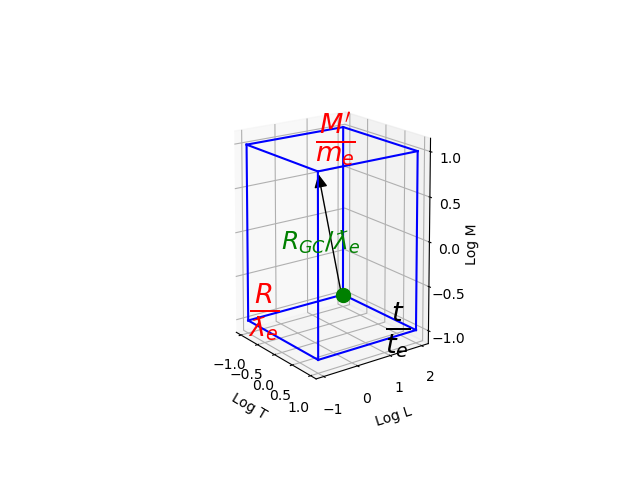
\includegraphics[width=5cm,height=6cm]{./figures/triaxis.png}
\caption{Geo dimensional Universe-Grandcosmos couple, with unit length The Electron Compton reduced wavelength. In a 3D Super-space, natural logarithms of physical ratios are considered vectors. The Grandcosmos radius appears as the norm of the vector using for length and time projections a common ratio, that of the Hubble radius, and for mass ratio $M^{\prime}$ byrespect to the electron mass. $M^{\prime}$ being the critical mass in the Grandcosmos reduced spherical hologram, this is a dramatic geometrical confirmation of the Extended (2D-1D) Holographic Principle applied to the Bekenstein-Hawking Universe entropy. The Grandcosmos existence cannot be denied since the relation involving $e$ and $a$ reach precision $10^{-7}$.} 
\end{figure}

Another crucial point in Physics is the existence of invariant fundamental constants. Thus, association of three of them must give characteristic values of $M$, $L$, $T$. So, approaching a domain in Physics necessitates to calculate characteristic values ($M, L, T$), from the three universal constants which are the most pertinent in the considered domain. This Prospective Dimensional Analysis is largely used in Fluid Mechanics, were the equations are intractable. However, is largely ignored in other domains because there is not really mathematical foundation, apart the above essential remarks. The triplet $c, G, \hbar$ which define the above Planck units is a notable exception. However, there is no interpretation for the Plack mass, except the fact it appears in Biology \cite{Sanchez1}. 

But, in virtue of the above Hierarchy Principle, the lack of theoretical justification is not a reason to
neglect Prospective Dimensional Analysis. 

The elimination of $c$ in the above $R$ formula means that the simplest basic dimensional
analysis starting from $\hbar$, $G$ and $m$, the Electron-Proton-Neutron mean mass, gives a good
approximation for $R/2$. Indeed, in the Hypothesis of a coherent Cosmos, it is logical to discard $c$
which is far two small a speed. This has not been observed during one century since $c$ is always
believed to be the single mandatory foundation of space-time. The warning of Poincar\'{e}, the true
discoverer of Relativity: `use 4D space, but do not confound Space and Time` has long been
forgotten, and physicists have unwisely put $c = 1$ in their equations.

In his three first minutes of cosmology, the first author obtained the length:
\begin{equation}
l \{\hbar,G,m\} = \hbar^{2} /Gm^{3} \approx R/2
\end{equation}
but it took nine years to get this published \cite{Sanchez3}, and it appeared later \cite{Sanchez1} that $m$ must be considered more precisely as the cubic root of the product 
$
m_{e} \cdot m_{p} \cdot m_{H}$

Moreover, the above critical condition
links the time $t = R/c$ and the mean mass density by the $c$-free formula:
\begin{equation}
\rho_{c} = 3/8\pi Gt^{2} \approx 9.41198 \times 10^{-27} kg \cdot m^{-3}
\end{equation}
Thus, the mainstream idea of a temporal variability of the mean density $\rho_{c}$ cannot be to
sustain, meaning that $\rho_{c}$ must be considered a fundamental constant. This writes:
\begin{equation}
t\{\hbar,\rho_{c} ,G\}\, = 1/\rho_{c}^{1/2} G^{1/2} = (R/c) (8\pi/3)^{1/2}.
\end{equation}
This idea of $\rho_{c}$ being a fundamental constant permits to define $R$ without any ambiguity: this is the 
radius of the sphere containing critical mass. This means each topon is the center of an equivalent black hole,
justifying the above application of the Bekenstein-Hawking entropy. 

Opponents would say that the
center of a black hole presents a singularity: that is indeed the case in the above flickering Space-
Mass-Time hypothesis. Other will argue that the flying galaxies cannot reach the celerity $c$ at
horizon, but it must be recognized that Relativity is a local theory, so do not apply to cosmology at large.
Indeed, even General Relativity in unable to define what is a Galilean frame, while the Foucault
pendulus shows it directly, realizing the Cosmic Microwave Background frame, identified with the
Grandcosmos frame, as seen above.

Introducing the Fermi constant $G_{F}$, the associated $c$-free length is very particular, to $1.7\%$:
$$l\{\hbar,\rho_{c},G_{F}\} = \hbar/\rho_{c}^{1/2} G_{F}^{1/2} \approx 9.07154 \times 10^{9} m \approx \lambdabar_{e}^{2}/l_{P}$$
Now, the following mandatory $c$-free times are close to each over $(0.7\%)$:
\begin{equation}
T\{\hbar,\rho_{c} ,G_{F} \}\, = \hbar^{4} /\rho_{c}^{3/2} G_{F}^{5/2} \approx 5.4829 \cdot 10^{57} s
\end{equation}
\begin{equation}
T^{\prime}\{\hbar,G,m\} = \hbar^{3} /G^{2} m^{5} \approx 5.5224 \times 10^{57} s
\end{equation}
One would conceive it as the periodic time of a Super-cycle, which matches Topological Axis at n = 30,
the holic dimension (see below), to 4\%. Comparing $T$ with the Kotov Non-Doppler Cosmic
Oscillation period $t_{K} \approx 9600.60(2)$ s, one observes, to $0.04\%$:
$$T/t_{K} \approx O_{M} /\sqrt{2}$$
where $O_{M}$, the cardinal order of the Monster Group, have been detected in the Section 2.3.1, again in relation with the Kotov period. Eliminating the later, this introduces the above $t_0$ chronon :
\begin{equation}
T/t_0 \approx (3/e\sqrt{2})O_M^3
\end{equation}
The simplest interpretation follows: this is the number of quantum events in a Super-cycle of period $T$, in a perfectly deterministic Cosmos. 

The  Monster  Group,  the largest of 26 sporadic groups, is suspected by some researchers to play a central role in Physics: indeed string theory allows a bridge between apparently no-connected mathematical theories \cite{Borcherds}. see below the dramatic properties of $O_M^3$.

Introducing the above Pioneer abnormal deceleration $g_{Pn}$, one gets the time: 
$
t\{G, m_{e} , g_{Pn} \} = (Gm_{e} /g_{Pn}^{3} )^{1/4} = (t_{Pn}^{3} t^{\prime}_{e} )^{1/4}
$, where $t_{Pn} = c/g_{PN}$ and $t^{\prime}_{e} = Gm_{e} /c^{3}$ . This time is compatible with:
\begin{equation}
t\{G, m_{e} , g_{Pn} \} = t_{K} /(F/a)^{2}
\end{equation}
where the above Tifft factor $F/a$ appears. The implication of the time 
$t^{\prime}_{e}\, = Gm_{e} /c^{3} = 2.2568 \times 10^{-66} s$
confirms the above Planck's wall breakdown.

\markright{F.M. Sanchez,\ V.A. Kotov,\ M. Grosmann,\ D. Weigel,\ R. Veysseyre,\ C. Bizouard,\ N. Flawisky,\ D. Gayral,\ L. Gueroult, \textit{Back to Cosmos}}
\section{The Arithmetical Logic: Holic Principle}
\markright{F.M. Sanchez,\ V.A. Kotov,\ M. Grosmann,\ D. Weigel,\ R. Veysseyre,\ C. Bizouard,\ N. Flawisky,\ D. Gayral,\ L. Gueroult, \textit{Back to Cosmos}}

In the hypothesis of an Arithmetic Cosmos, the ultimate equations must be diophantine. The
simplest one is $T^{2} = L^{3}$, where $T$ is a time ratio and $L$ a length one, resolved, since 2 and 3 are 
co-prime, by $$T^{2} = L^{3} = N^{6}$$ where N is a whole number, meaning the classical 6D space of classical point mechanics. Considering the exponents, this particularizes the usual 3D space, but attribute 2 dimensions for the Time, in conformity with an independent study \cite{Bars}.

This is the degenerate arithmetic form of the spatio-temporal holographic principle.

This is also the 3rd Kepler's law, but its diophantine form gives $L = n^{2}$, the orbit law in the Hydrogen atom and in our
Gravitational Molecule model, where the visible Universe corresponds to the first orbital,
suggesting the existence of a Grandcosmos, as the Topological Axis does also, which favors the
dimension n = 30, the natural extension of the above:
\begin{equation}
T^{2} = L^{3} = M^{5} = N^{30}
\end{equation}
where $M$ is a mass ratio. Recall that the lifetime of an unstable particle depends on the 5th power of its mass. This holic dimension 30 is the touchstone of the Topological axis, from which gauge bosons are deduced by Bott reductions [19] (Fig. 1)

This is called the Holic Principle, relating to the apparent world. The Complete Holic
Principle \cite{Sanchez4} involves a field term $F^{7}$, and so introduces the dimension $30 \times 7 = 210$. It is confirmed by (to 15 ppm, 1.1 ppm, 56 ppm):
$$2/\delta \approx (R/\lambdabar_{e})^{1/210} \approx (1/2d_{e}) ln(pH)/lna \approx (1/d_e^{2})ln\tau/ln\mu$$
where appear the masses of the heavy leptons (Section 9.5). This implies a dramatic geo-combinatorial relation between $a$ and $p$ : $p^{p^{2}} \approx (a^{2})^{a^{3}}$ and confirms the central computational role of $\delta = R^{\prime}/R = pH/a^{3}$, which is to 1.6 ppm:$\delta \approx e^{2/e^2}$, confirming the central role of $e$ (section 9.1).

\markright{F.M. Sanchez,\ V.A. Kotov,\ M. Grosmann,\ D. Weigel,\ R. Veysseyre,\ C. Bizouard,\ N. Flawisky,\ D. Gayral,\ L. Gueroult, \textit{Back to Cosmos}}
\section{The special holographic relations}
\markright{F.M. Sanchez,\ V.A. Kotov,\ M. Grosmann,\ D. Weigel,\ R. Veysseyre,\ C. Bizouard,\ N. Flawisky,\ D. Gayral,\ L. Gueroult, \textit{Back to Cosmos}}

The holographic technique is by far the most efficient way to treat huge information \cite{Grosmann}, based on the
properties of a coherent wave. Now, the main lesson of modern physics is that everything (light \textit{and matter}) propagates by waves  (quanta appearing only at the detection). Moreover, a coherent wave is represented by a unitary matrix of quantum mechanism: we haven shown that the quantum formalism is very similar to the holographic one, describing an interaction by a two-step holographic process. From these considerations a mass for the photon (confirmed in section 4.1) and graviton has been proposed \cite{Sanchez1}, and are indeed in definite places in the Topological Axis (fig. 1)

A Holographic Principle has been coined by some theoreticians \cite{Bousso}, the name coming from the idea of dimension reduction, from 3D to 2D, similar to the visual impression in current visible holograms (in fact holography is only the 2D restitution of a propagating wave). It this respect, it is strange that no one tried to extend this process to 1D (an idea of temporal holography proposed in the author's thesis in 1975): this is the subject of Section 3, but using only the Planck length and the topon. It is natural to suppose that they are other holographic wavelengths. In fact \textit{the Topological Axis is the reunion of height 1D-2D holographic relations}. We present here three more significant examples. 

\subsection{The Conservation of Information}

The Grandcosmos holographic reduction radius $R^{\prime}$ shows itself an overwhelming holographic
relation with the CMB Wien wavelength $l_{CMB} = hc/kTw $, with $w = 5 (1-e^{-g}) \approx 4.965114245)$ to $0.01\%$:
\begin{equation}
4\pi(R^{\prime}/l_{CMB})^{2} \approx e^{a}
\end{equation}
Since the holographic technique uses coherent radiation, this seems incompatible with the CMB
thermal character. But \textit{in a totally deterministic cosmos, there is no paradox}. This question is
connected with the black hole information paradigm \cite{Preskill}. Independently of our approach, an
argument in favor of a total conservation of information was tied to a non-evolution cosmology
\cite{Nikolic}. 

Note that $e^{a}$ is also compatible with the half volume of the proton, with
the Planck length as unit.

So, while General Relativity and Unitary Quantum physics disagree about the nature of Space-Time, especially the non-locality phenomena, they agree for complete determinism, leading to the collapse of the
Copenhagen statistical interpretation. The hidden variables exist really: it is the Cosmos ! Heisenberg
relations would be only Fourier transform manifestations of Wave Mechanics.

The wien wavelength enters (0.03 \%):
\begin{equation}
l_{CMB} / \lambdabar_e \approx P/pH a^3
\end{equation}
showing evidence for the invariance of the cosmic temperature, and confirmed in the following section. 

\subsection{The Cosmic Temperature}

In the gravitational hydrogen molecule model, $R$ is defined by the following 1D-2D Special
Holographic Relation, using the wavelengths of the electron, proton and hydrogen, while the background wavelength appears in the 3D term involving the molecular Hydrogen wavelength:
\begin{equation}
2 \pi R/\lambdabar_{e} = 4 \pi \lambdabar_{p} \lambdabar_{H} /l_{P}^2 \simeq (4\pi/3)(\lambdabar_{CMB} /\lambdabar_{H2})^{3}
\end{equation}
The above relation gives $T_{CMB} \simeq 2.73 K$. With the measured temperature of the cosmic
background, there is a small gap compatible with $(H/p_G)^2 p/6\pi^5 $, where $p_{G}^{2} = P^{2} /2^{127}$ , with $P = \lambdabar_{e} /l_{P}$. 
This eliminates $l_{P}$, producing a relation independent of $G$, implying $T_{CMB} \approx 2.725820805$ Kelvin:
$$2^{127} = 2\pi^{2} \lambda_{CMB}^{3} /\lambdabar_{e} \lambdabar_{H}^2$$
which is the area of the 4-sphere of radius $\lambda_{CMB} / \lambdabar_{m}$, where $\lambdabar_{m} = (\lambdabar_{e} \lambdabar_{H}^2)^{1/3} $ proving the relevance of
the Lenz-Wyler approximation for the Proton/Electron mass ratio $p = 6\pi^{5}$, (see Section 9.2). Recall
that $2^{127} - 1$ is the most famous prime number in the history of Mathematics, being the last term of
the Combinatorial Hierarchy \cite{Sanchez1} of special imbricated Mersenne numbers 3, 7, 127, the sum of which is 137.

\subsection{The Holic Principle and Cosmic Coherent Oscillation}

While the HB entropy of the sphere of radius $R^{\prime} = 2r_e^3 / l_P^ 2$, where $r_e = \lambdabar_e /a $ is the electron classical radius, which is the holographic reduction of the Grandcosmos (section 3), verifies the relation:
\begin{equation}
\pi(R^{\prime}/l_P)^2 = (pi/2)(R^{\prime}/r_e)^3 
\end{equation}
with a wrong geometric coefficient, the HB entropy of the visible Universe shows a nearly geometric term, with imprecision $\sqrt{4/3\delta} \approx 0.17$:
\begin{equation}
\pi(R/l_P)^2 \approx (2\pi/3)(R/r_e)^3 
\end{equation}
which is a holographic conservation concerning \textit{the half-sphere of the visible universe}. By analogy with the above scanning process filling the whole sphere (section 3), the above Kotov length $l_k$ (section 4.3) permits to introduce two holographic relations, involving the whole sphere (0.90 \% and 2.6 \%):
\begin{equation}
\pi(R/l_K)^2 \approx 2\pi l_K/r_e 
\end{equation}
\begin{equation}
(4\pi/3)(R/l_K)^3 \approx 4\pi (r_e/l_P)^2 
\end{equation}

The deviation of Eq. (28) is very close to that of Eq.(10), inducing, to 17 ppm and 13 ppm: 
\begin{equation}
 (R_{GC}l_P/Rr_e)^2 \approx (R_1l_K/Rr_e)^3 \approx \mu^{35}(p/H)^2/ln2
\end{equation}
showing a holic form, involving the Muon/Electron mass ratio $mu$ (see section 9.5).
Taking account of the identity: $2l_P^2 = \lambdabar_M R = (R^{\prime}r_e)^2/(R_GC)l_P)^2$, this leads to a number reduced in the ratio $\delta^3$, where the fourth root shows the Koide constant $p_K$, characteristic of the two Heavy Leptons (Eq. 68) (17 ppm and 1.8 ppm) :
\begin{equation}
r_/\lambdabar_M \approx (R_1l_K/R^{\prime}r_e)^3 \approx (4\pi P/p_K)^4
\end{equation}
The above term $R_1l_K/R^{\prime}r_e$ is close to (1\%) $\sqrt{O_M} \approx 2a^2P$ (0.18 \%). The study of deviations shows the intermediate bosons ratios $W$ and $Z$, with values specified to the ppb range in section 9.4, leading to (-4 and 3.5 ppm):
\begin{equation}
O_M (FR^{\prime}/PR_1)^2 \approx W^4 (137/a)^3
\end{equation}
\begin{equation}
 (F^3R_1 / 2 a^3R^{\prime})^2 \approx Z^4 (a/137)(p_0/p)^2
\end{equation}
Thus, (0.3 and -0.4 ppm)
\begin{equation}
137 p_0 W^2 Z^2/p a_w^2 \approx \sqrt{O_M}/(2a^2 P) \approx e^{-4a}
\end{equation}
this precises a known relation in Particle Theory.

\markright{F.M. Sanchez,\ V.A. Kotov,\ M. Grosmann,\ D. Weigel,\ R. Veysseyre,\ C. Bizouard,\ N. Flawisky,\ D. Gayral,\ L. Gueroult, \textit{Back to Cosmos}}
\section{The role of Intermediary Mathematical Constants}
\markright{F.M. Sanchez,\ V.A. Kotov,\ M. Grosmann,\ D. Weigel,\ R. Veysseyre,\ C. Bizouard,\ N. Flawisky,\ D. Gayral,\ L. Gueroult, \textit{Back to Cosmos}}

\markright{F.M. Sanchez,\ V.A. Kotov,\ M. Grosmann,\ D. Weigel,\ R. Veysseyre,\ C. Bizouard,\ N. Flawisky,\ D. Gayral,\ L. Gueroult, \textit{Back to Cosmos}}
\subsection{The Eddington's constant 137}

The initial Eddington's proposal for $a$ was the whole number 136, as the number of independent parameters in the symmetric matrix $16 \times 16$. Note that \textit{n = 16 is the central dimension of the Topological Axis}. Later, one unity was added, becoming 137, a number which intrigued many physicists for a century, but apparently nobody highlighted it has a fundamental mathematical property: it appears as a Singular Prime in the series of the maximal primes appearing in the numerator of the harmonic
series: 3,11,5,137,7,11, showing a symmetry between the 11 dimensions of M theory (a synthesis of five string theories) and the 4 of space-time. Indeed: $137 = 11^{2} + 4^{2}$, while, as seen above:$11/4 = (\lambda_{CNB}/\lambda_{CMB})^{3}$

Since Riemann series are tied to the prime number distribution, it seemss odd and incredible that mathematicians
have not point out the primes appearing in the harmonic series since it is the single pole. It seems
that the basic precept `all occurs in the pole` was forgotten in this case. 

As ancient Egyptians used only fractions of type $1/n$, they were certainly aware of this particular harmonic series: 
$S_{5} = 137/60$
Indeed it appears in the Ptolemaic approximation for $\pi$: $\pi_{Pt} = 377/120 = 2 +  S_{5}/2$.

Recall that the electrical constant $a$ characterizes the force $$F =\hbar c/al^{2}$$ between two l-distant
elementary charges, where $a$ appears central in Atomic Physics and in many fine-tuning relations \cite{Carr}. It is
misleading that physicists focused on one property only, the appearance of its fifth power in the
Hydrogen hyper-fine spectra, and call its inverse $\alpha$ the `fine-structure constant`. It is strange also that
Eddington's Theory was rejected as soon as $a$ appeared to deviate from 137. Indeed, the
following shows that 137 plays a central role in fine-tuning analysis. 

One may interpret 137 + 1 as
the sum of the numbers of dimensions in the Topological Axis \cite{Sanchez1}, taking into account the double
point (H atom-Pion couple) for the superstring value n = 10, and the remarkable sum:
\begin{equation}
\sum_{k=7}^{k=0}(2 + 4 k ) = 2^{7}
\end{equation}
So $137 = 2^{7} - 1 + 3 + 7$ the Combinatorial Hierarchy form \cite{Sanchez1}. But this appears also as 137 = 135 + 2,
with the dimension 2 of the String patent. In particular, one obtains the value $a \approx 137.035999119$
compatible with measurement $a \approx 137.035999139(31)$ in:
\begin{equation}
ln137/ln(a/137) \approx (2+135/d_{e})^{2}
\end{equation}
meaning the ratio $a/137$ acts as a canonical ratio. Indeed, the Bizouard constant $f$, precising \cite{Sanchez1} the inverse of the standard 'strong coupling constant' 0.1184(7): $$f = a_w/2\pi(pH)^{3/2} \approx 8.43450$$ appears as a computation basis, in the following dramatic relations, to 0.3, 0.2, 0.7 \% and 22 ppb ! (confirmation of $G$ value):
$$(a/137)^F \approx 3^a \approx f^{f^2}/\pi \approx (O_B/f)^2 \approx P^4 (2/3)^a (p/p_0)^2 $$
proving that the base 3, \textit{the optimal whole number basis}, is also used by the Cosmos as well as $O_B$, the cardinal order  of the Baby Monster (as confirmed below). 
Note that while $R/\lambdabar_e \approx 2^{128}$, to 0.6 \%, $R^{\prime}/\lambdabar_e \approx 27^{27}$, with $27 = 3^3$ to 0.03 \%  Moreover, to 27 ppb:
$$ a/(a-1) \approx 3^{1/150} $$
Thus, the basis 3 makes a liaison between $a/137$ and $a/(a-1)$, very close (2 ppm) to the Bond factor 137/136, central in Eddington's theory \cite{Eddington}.

\subsection{The Atiyah and Sternheimer constants}
    Sir Michael Atiyah was a precursor in the search for unity in Mathematics and Physics. His last work in this domain introduced the constant $$\Gamma = \gamma a /\pi$$ as a simplification term \cite{Atiyah1}. Indeed $\Gamma$ and the canonical $e^{\pi}$ enter the following dramatic simplification of the above (Section 4.1) single-electron cosmic formula (0.3 ppm):    
\begin{equation}
a = (p/H)((ln(R_1/\lambdabar_e) + \gamma – 1)/(\pi^2/6 - 1)) \approx ln(R/\lambdabar e) + \Gamma + e^{\pi}
\end{equation}
so confirming the $R$ value to 45 ppm, a correction which is $\beta p/p_0$, within 0.2 ppm.

Moreover, this confirms the central role of the Sternheimer scale factor $j = 8\pi^2/ln2$ (to 0.013 \%, 0.013 \% and 0.046 \%):
\begin{equation}
j \approx ln(R/\lambdabar e) + \Gamma \approx a - e^{\pi} \approx e^{\pi} lna
\end{equation}
It was noted \cite{Sanchez1} that $$j\approx T_{mam}/T_{CMB}$$ the ratio between mammal and cosmic temperatures, and that the mammal wavelength enters (1\%) $$(Rl_P)^{1/2}\approx hc/kT_{mam}$$ So, \textit{the couple thermal photon-Life is at the upper center of the Topological Axis}, while the down center is the Higgs boson (Fig.1). The real center, as seen above, is the dimension $n = 16$. Moreover, to 0.1\%, the water triple point enters: $$(R^{\prime}l_P)^{1/2}\approx hc/kT_{H2O}$$ which is also the product of triple points of Hydrogen and Oxygen, divided by the cosmic temperature. This shows that Chemistry is also involved \cite{Sanchez1}.

Now, the study of the 22 amino-acids \cite{Sanchez1} has shown that $j$ is a computation basis. Indeed, to 2\%: $j^{22} \approx 3 P^2 $ and, more precisely, to 0.01 \% :$j^{22} \approx Pp_E^7 $ where $ p_E \approx 1847.599459$ is the Eddington's mass ratio of the couple proton-electron, the roots ratio in the Eddington's equation $10x^2 - 136x + 1 = 0 $.

The last equation means the implication of $B = e^{e^{\pi}}$, the double exponential of $\pi$, in the ultimate theory. Indeed, to 0.3 ppm and 0.03 \% :
\begin{equation}
(\lambdabar_{CMB}/\lambdabar_e)^3 \approx F^5/6 \approx B^3/a
\end{equation}
It is also exhibited in the following holographic relation:
\begin{equation}
(4\pi/3) B^3 \approx \pi(F^3/a)^2,
\end{equation}
while $F^3/(44\pi)$ is close, to 0.01 \%, to the term $A = (3/2) a^7$, which enters the 'forgotten' electromagnetic power $E_e^2/\hbar A$, in the Hydrogen atom, with $E_e = m_ec^2$.
Note that, to 10 ppm and 2 ppm:
$
(H/n)^2(F^2/B)^3 \approx (4/3) a^2 \approx W/2\pi \beta^4
$
where $W$ is the W boson-Electron mass ratio (see Section 4). Now, to 30 ppm and 20 ppm :  
\begin{equation}
 (F^3/a)^2 \approx (P/FH^2)^3  \approx  (a/137)(4\pi/3)(F^2/p^{1/2})^3 
\end{equation}
Thus, the term $F^3/a$ seems special. More precisely, with the reduced Hydrogen radius $a^{\prime} = aH/p$, to 0.3ppm and 0.3 \%:
\begin{equation}
\sqrt{\beta} F^3/a^{\prime} \approx (e/3)(e/2)^j  \approx (3/\pi) 4^{\Gamma}
\end{equation}
confirming that $j$ and $\Gamma$ are generalised dimension, i.e., as privileged exponents, calling for further study.

Note that (Fig 1.):
\begin{equation}
m_{e} c^{2} f(\gamma\Gamma) \approx 125.175 GeV
\end{equation}
seems compatible with the Higgs Boson energy, matching with the dimension index $k \approx \pi$, leading to $$\gamma\Gamma \approx (4\pi + 2) (p/d_e p_0)^2 $$ to 30ppb.
The length $\lambdabar_{e} f(\Gamma) \approx 5\times 10^{5}$ light-years is characteristic of a galaxy group radius, and $c$ times the Milankovich period. One observes also, to 0.16 \%, 1.8 ppm and 10 ppb:
$$e^\pi \approx (\Gamma - 2)/d_e \approx a_w^{1/f}/d_e^2 \approx (16/ln2)d_e \beta p/p_0$$
meaning that the special value in the Topological Axis $k = e^{\pi} /4 \approx 4/ln2$ corresponds to $n \approx \Gamma$.
One notes also, for the Pions mass ratios, in their 5 ppm uncertainty:
$$a/\pi\approx 496^2/137\Pi_0^{2/3} \approx p\beta^2/\Pi_+^{2/3}\approx (a/137)^{1/2} F^{10/3\sqrt{a}}$$
(1.8 ppm), confirming Atiyah's symmetry between $\pi$ and $a$, the role of the dimension 496, and the pertinence of the $20^{th}$ power of $F$, corresponding to the 20 normal amino-acids.  

\subsection{The ubiquity of $a^{a}$}
\markright{F.M. Sanchez,\ V.A. Kotov,\ M. Grosmann,\ D. Weigel,\ R. Veysseyre,\ C. Bizouard,\ N. Flawisky,\ D. Gayral,\ L. Gueroult, \textit{Back to Cosmos}}

From the Computation Hypothesis, $a$ must be an optimal basis, and, as seen above, 137 being is a number of parameters in the Eddington matrix, it must be interpreted as a dimension, a privileged exponent. \textit{So the term $a^a$ must be central}.
    
Indeed, $a^a$, apart a $\pi$ factor, is the Grandcosmos volume with unit length the Hydrogen radius, to 0.4 and 0.5 \%:
\begin{equation}
(4\pi/3)(R_{GC}/r_H)^3 \approx a^a/\pi \approx 3(1/ln2)^{\sqrt{pH}}
\end{equation}
Note that the ln2 factor involves information theory.
Moreover, the dramatic relation $a^a\approx e^{p/e}$ has been connected with the fifth optimal musical scale (306 notes) and to the operational definition of $e$ \cite{Sanchez1}. Thus it seems interesting here to look for its manifestations in classical mathematics. 

The famous Lucas-Lehmer primality test uses the series of whole numbers $N_{n+1} = N_{n}^{2}-2$,
starting from $N = 4 = u_{3} + 1/u_{3}$ , with $u_{3} = \sqrt{3} + 2$, belonging to the Diophantine generators $u_{n} = \sqrt{n} + \sqrt{(n+1)}$, which entire powers are close to whole numbers. One shows that $N_{n} \approx u_{3}^{(2^{n})}$, and for n = 9:
\begin{equation}
u_{3}^{2^9} \approx (2(137^{2} + 48))^{64} \approx a^{a}
\end{equation}
defining $a$ to 39 ppm and showing that the Rydbergh term $2a^2$ plays a central role (see Eq.(33)).

Also, with the Pell-Fermat generator $u_{1} = 1 + \sqrt{2}$:
\begin{equation}
a^{a} \approx u_1^{3\times(2^{8}-1)}
\end{equation}
which defines $a$ to 0.3 ppm. So the number $a$ establishes a connection between $u_{1}$ and $u_{3}$, two of the
simplest arithmetic's generators. This opens a \textit{new research in pure mathematics}.

Remark that the $12^{th}$ Pell-Fermat number is $ u_1^{12}/2 \approx 140^2 + 1 \approx a(a+6)$ to 4 ppm. So, this comes back to the antique problem of the rationalisation of $\sqrt{2}$. Its correct value shows a $8^{th}$ fractional term very close to $\sqrt{5}$, so leading to $\sqrt{2}_a \approx N_{a}/D_{a}$, with $ N_{a} = 239 \sqrt{5} + 99 \approx \Gamma^{2}
\approx O_B^{1/12} $ and $ D_{a} = 13^2 \sqrt{5} + 70 \approx O_M^{3/61}$,
so connecting $O_M$ and $O_B$, since $61/2 \approx F/a^{2}$ to 0.04 \%, and introducing the next section.

\subsection{The intervention of Sporadic Groups}

With the tachyonic ratio $Q = R_{GC}/R = C/c$, the cardinal orders of the two giant sporadic groups enter (63 and 2 ppm)
\begin{equation}
\pi Q/a \approx O_M D n/H \approx O_B P a^{3/2}
\end{equation}
where $D = 196883$ is the Moonshine dimension of the Monster group.
The above term $O_M^3$ appears in (0.08\%, 2.5\%,1\%, 2\% and 61 ppm):
\begin{equation}
e^{137e}\approx (e/3)e^{ea}\approx O_M^3 \approx 496^{60} \approx fe^{16e^\pi} \approx f^{4d137/\pi}
\end{equation}
implying the Green-Schwarz string dimension 496, which is the third perfect number, after 6 and 28, and tied to the Brout-Englert-Higgs boson in the Topological Axis (Fig.1). The above Bizouard constant confirms it is a computation basis, and the above relation implies, to 61 ppm:
\begin{equation}
lnf\approx \pi e/4d_e
\end{equation}
The following combination of three main dimensionless parameters is remarkable: they are the electrical
one $a$, the Fermi ratio $F =\sqrt{a_{w}}$ and the strong Bizouard ratio $f$, to 0.05 \% and 0.13 \%:
\begin{equation}
F/af \approx 496\approx j^{\delta}
\end{equation}
Also, to 8 ppm: $$\ln(O_{M}) /2\ln\ln\ln\ln(O_{M}) \approx 137$$ and the product of the 20 groups of the happy family tied
to the Monster shows, to 0.015\%, 1\% and 0.9 \%:
\begin{equation}
\Pi_{happy} \approx \delta \times a^{a} \approx j^{j^{\pi/3}} \approx (j/496)^2 \Gamma^{210}
\end{equation}
This confirms the above Complete Holic Principle, and the computation basis role of $\Gamma$ is moreover confirmed by, to 2\%: $$a^a \approx \Gamma^{209}$$ and the order of the Baby-Monster $$O_B\approx\Gamma^{24}$$ Now, from $209 = 137 + 3\times 24$:
\begin{equation}
O_B \approx (a/\Gamma)^{a/3}
\end{equation}
where $a/\Gamma = \pi/\gamma $ is the canonical Atiyah ratio.

The total product of the 26 sporadic orders $\Pi_{26}$ verifies, with n the neutron/electron mass ratio, to 1.8 ppm:
$$ \Pi_{26} \approx (9np_0/2p^2)(R_{GC}/\lambdabar_M )$$
Now $\Pi_{26}$ is close to $e^{4 \times 210}$, whose $a^{th}$ root is again very remarkable (65ppm, 98 ppm, 5 ppb):
\begin{equation}
e^{4 \times 210/a} \approx 2e^{2e} \approx H/4 \approx 26 \times (2 \times 26 + 1)/3
\end{equation}
The ppb range precision of the last term means clearly that a rationalisation of $e^{2e}$ is occuring, where the canonic dimension 26 plays a central role.

Note that, in Eq.(40), $j/496 \approx 0.229$ is close to the weak mixing angle, but $p/g_0 \approx 0.232$ is closer to the measured value 0.23116(12) \cite{Tanabashi}, where $g_0 = 7920 $ is the smallest Matthieu sporadic group order. These ratios appear as calculation basis in the product of cardinal orders of the Monster and the baby-Monster groups, to 1\%, 0.2 \%, 1 \% and 0.7\%:
\begin{equation}
O_MO_B\approx H^{2H/a} \approx (g_0/p)^a \approx (496/j)^{137} \approx \sqrt{2}(e496^2)^{15}
\end{equation}
confirming the central role of 496. Note also (0.1 \%) that $O_MO_B \approx  n_{ph}/\delta^{1/2}$, where $n_{ph}\approx (3/\pi) exp(e^6/2)$ (to 0.2 \%) is the photon number in the visible universe. 

From the Eqs (38), (42) and (44), by taking the $137^{th}$ root, one obtains, to 0.03 \%: $496/j \approx (ae^e/\Gamma)^{1/3}$
Now $ae^e/\Gamma$ is close to $2ed_e$. More precisely (0.7 ppm):
\begin{equation}
a/\Gamma = \pi/\gamma \approx 2d_e \times e (p_0/p)^2 
\end{equation}
Thus, \textit{the Atiyah symmetry infers a relation between the three mathematical constants $e$, $\pi$ and $\gamma$ and the Electron magnetic moment $2d_e$}. It is remarkable that this is obtained from singularities involving the two Monster groups. This introduces the next section.

\markright{F.M. Sanchez,\ V.A. Kotov,\ M. Grosmann,\ D. Weigel,\ R. Veysseyre,\ C. Bizouard,\ N. Flawisky,\ D. Gayral,\ L. Gueroult, \textit{Back to Cosmos}}
\section{The Fine-tuning with basic mathematical constants}
\markright{F.M.Sanchez,\ V.A.Kotov,\ M.Grosmann,\ D.Weigel,\ R.Veysseyre,\ C.Bizouard,\ N.Flawisky,\ D.Gayral,\ L.Gueroult,\ Back to Cosmos}
\markright{F.M. Sanchez,\ V.A. Kotov,\ M. Grosmann,\ D. Weigel,\ R. Veysseyre,\ C. Bizouard,\ N. Flawisky,\ D. Gayral,\ L. Gueroult, \textit{Back to Cosmos}}

Since some dimensionless physical parameters are very precisely measured, we looked for
relations with mathematical constants such as $e$, $\pi$ and $\gamma \approx
0.577215665$, the Euler-Mascheroni constant, which appears already in the above single-electron
cosmic radius and the Topological Axis.

\subsection {The optimal calculation base $e$ confirmed}

The Topological Axis shows clearly that the Grandcosmos is defined by the following conjunction (1\%):
\begin{equation}
f(k = e^{2}) = exp(2^{e^{2+1/2}}) \approx exp(e^{2e}+e^{2})
\end{equation}
where the supplementary term $exp(e^2)$ is close to $a^{3/2}$. Note these properies of the 'economic number', to 
0.4 \%, 6 ppm, 0.4 ppm,0.3, 0.04, 0.4, 0.2, 0.6 \%:
$$
\begin{array}{ll}
%
\displaystyle
e^{e^e}\approx (lnp)^{lnp}  
\approx 137 (e^{e})^3 \approx e^e a \sqrt{pH} (p/p_0)^2 \approx j^6/F \\
\approx FlnD/ln(2\pi) \approx FlnF/2 \approx 2WlnZ \approx Zln(\lambdabar_{CMB}/\lambdabar_e) 
\end{array}
$$
Note that $e^2$ is the limit of the following musical series:
$$(3/2)^5 \approx (4/3)^7   \approx (5/4)^9  \approx  (6/5)^{11}  \approx   ...  \approx  (1+1/n)^{2n+1}  $$  
a series converging very much rapidly than the classical Euler's one $(1+1/n)^n$. The first two terms defines the occidental 12 tones scale.

The canonical ratio $R_{GC}/\lambdabar_M = 2P^9/a^6pH $ confirms the Extended Holographic Principle, to 0.04 \%:
\begin{equation}
R_{GC}/\lambdabar_M  \approx (137e/a)^{420}  
\end{equation}
exhibiting the following property (0.3 ppm):
 $$ (a/137)^{420} \approx (137 - 3)/120 $$  
with $137 - 3 = 7 + 127$ are the Combinatorial Hierarchy terms, 

\subsection {Lenz-Wyler's Formula}
Armand Wyler singularized a value approaching $a$ to 0.6 ppm and confirmed the pertinence
of the Lenz approximation which plays a central role above: $p_{0} = 6\pi^{5}$ approaching $p$ to 18.824 ppm.

A confirmation of a symmetry between $a$ and 137 is the following relation involving $H$, the
Hydrogen electron mass ratio, precise to 83 ppb:
$$a/137 \approx (p_0 H)^{1/2} /p$$
One observes that the rejection of Wyler's work, due to a non-perfect formula for the $p$ and $a$ values, is a new
manifestation of the general neglectance of the Principle of Hierarchy.

A confirmation of a symmetry between $a$ and 137 is the two following approximations for $p$ with the same imprecision 80 ppb, so leading to the ppb relation:
 $$p \approx (137/a) (p_0 H)^{1/2}  \approx EH^3/d_e^2jFD $$ 
where $D = 196883$ is the Moonshine Monster dimension \cite{Conway}, which appears also, to $10^{-7}$, to be $(\pi_p P/d_eF)^{1/2}/H$, with $\pi_p = (p/6)^{1/5}$, so confirming again the pertinence of Wyler's approach. 

Note also that the Lenz-Wyler formula is nothing but the product of the area by the volume of a cube with side $\pi $. If one consider a cube with side 5, privileging again the identification dimension = exponent, this gives $6 \times 5^5 = 137^2 - 19 $. This is not a chance coincidence, because this relation has long time been deduced from basic considerations on quarks \cite{Sanchez1}. Indeed with $u = 5 $ and $d = 6 $, the combination $uud = 150 $, which power 3/2 is close to $H$, while the combination $udd \approx (n/a)^2 $. This leads to (0.012 \%) $6\times 5^5 \approx (aH/n)^2 $  
Note that, with $q = 2^{12}$ to 0.03 \%, 2.5 \% and 41 ppm:
$$R_{GC}/\lambdabar_e \approx q\times 5^{137} \approx 6^{137}/q^2 \approx 6^{128}/(1+1/\sqrt2)$$
Since $R/\lambdabar_e \approx 2^{128}$, the decomposition of 6 leads to a natural Universe-Grandcosmos partition, and to the following approximation for the tachyonic celerity ratio (0.01\%) 
$$ C/c\approx3^{128} (p_K/p_G \delta)^2 $$ where $p_K$ is the Koide constant (see section 9.5). This confirms the role of the correspondance quark up = 5 and \textit{quark d = 6 with a double structure}. It is an example of \textit{immergence}, i.e. deducing the small from the large, in a striking similitude between cosmology and nuclear physics. Another example was encontered in section 2.4, where dimensional analysis gives the visible Universe radius, in an easier way than the equivalent one for the Hydrogen atom radius, since for this case there is no evidence that $c$ must be left out.
Elimination of $q$ leads to (2.6 \%):
$(R_{GC}/\lambdabar_e)^3 \approx 150^{137}$. 

In Atiyah's last work the Bernoulli function $x/(1-e^{-x})$ is used. This is the kernel of the thermal Planck law. Indeed, considering the Wien reduced constant $w = hc/kT\lambda_{Wien} = 5 (1-e^{-w}) \approx 4.965114245$, one notes that $a \approx e^w -2\pi$, suggesting $a$ to be a trigonometric line. Indeed $cosa \approx 1/e$, and, to 65 ppb:
\begin{equation}
a \approx 44\pi - Arccos(1/e)
\end{equation}
a formula largely diffused on the web, but without indication of its origin. Now $w^{e^w}$ enters (1 ppm):
$$w^{e^w+1} \approx \sqrt{ad\sqrt{n/p}}R_{GC}/\lambdabar_e $$
This confirms that the Planck thermal law will play a central importance in the future fundamental theory. 

\subsection {The Archimedes constant $\pi$ as a calculation base}
\markright{F.M. Sanchez,\ V.A. Kotov,\ M. Grosmann,\ D. Weigel,\ R. Veysseyre,\ C. Bizouard,\ N. Flawisky,\ D. Gayral,\ L. Gueroult,\textit{Back to Cosmos}}

The value of the Topological Function for the main String
 dimension 26 renders, to 0.1\%, the same Lenz-Wyler form $f(26) \approx 6(2\pi^{2} a^{3} )^{5}$, where $2\pi^{2}a^{3}$ is the area of a 4-sphere of radius $a$. Moreover, with $n/p$ the mass ratio Neutron/Proton, to 0/3\%, 0.02\% and 1ppm:
$$(p/n) (R/\lambdabar_{e})^{2} \approx (f(26)/6)^{2} \approx (2\pi^{2} a^{3})^{10} \approx \pi^{155}$$
The corresponding value of $\pi$ in the last expression shows the fractional series 3, 7, 16, -u, with $u \approx
2 \times 137$, confirming again the Rationalisation Hypothesis. This leads to the rational value
\begin{equation}
\pi_{R} = (355u-22)/(113u-7) 
\end{equation}
This corresponds to the above $G$ value to 10 ppb accuracy.
Since $(R/\lambdabar_{e})^{2}$ is also close to $2^{256}$, within 1\%, this illustrates the following musical relation involving again 137:
$$2^{1/155} \approx \pi^{1/256} \approx (2\pi)^{1/3 \times 137}$$
The scale with 155 notes is not known, but 137 appears also in the classical musical scales \cite{Sanchez1}. 

whole powers of $\pi$ appears in the 2 ppm Reilly formula: 
\begin{equation}
a \approx 4\pi^{3} + \pi^{2} + \pi \approx \pi^{9/2}2^{-1/3}
\end{equation}
and recall that whole powers of $\pi$ appears also in the even order Riemann series.

\subsection {The Four Forces Unification in ppb Fine-Tuning}
The Particle standard model achieved the unification between electromagnetism and weak nuclear force, with propositions for extension towards strong nuclear force in Grand Unification Theory (GUT), but no synthesis have been possible with gravitational force. The Topologocal Axis shows clearlty that GUT with $1O^{16}$ GeV gauge boson seems confirmed. However, in section 4.2, it is proven that the Kotov oscillation reveals a symmetry between two apparently inconciliable domains: electroweak and gravitational forces. So we look here for a precise relation involving the 4 force parameters, $a$ (electric), $a_w$ (weak nuclear), $f$ (strong nuclear) and $a_G$ (gravitation). The later force is equivalently represented by $p_G = P/2^{127/2}$, with $P = m_P/m_e$, which was admitted to be:
\begin{equation}
p_G = \sqrt{pH} (p/H)^3/d_e
\end{equation}
 With the Atiyah constant $\Gamma = \gamma a/\pi$ is (section 8.2), we first noted that, inside the 250 ppb indetermination:  
 $a_{w} = F^2 = (137 \times 2 \Gamma)^{3}$
 which affects the form of the simplest diophantine equation (section 6).
 Now $a_{w}$ is a cube: $a_{w} = (\lambdabar_{e}/l_{eF})^{3}$, with $l_{eF} = (G_{F}/m_{e} c^{2})^{1/3}$. Thus:    
\begin{equation}
\lambdabar/l_{eF} \approx 137 \times 2\Gamma
\end{equation}
leading to:
\begin{equation} 
F = a_{w}^{1/2} = E_{F} /m_{e} c^{2} \approx 573007.3652
\end{equation}
This relation is so striking that we ask the computer if it can find synthetic precise relations involving the other forces parameters, in function of $\pi$ and $\Gamma$. Indeed, with the neutron/electron mass ratio $n \approx 1838.68366089(17)$, the computer gives the following relation in the ppb range:
\begin{equation}
aF/\sqrt(pH) \approx \pi(4n/\Gamma)^3/p_G \approx \mu^2
\end{equation}
where $\mu$ is the Muon/Electron mass ratio, \textit{inside its 20 ppb indetermination}, so proposing the value:
\begin{equation}
\mu \approx 206.7682869
\end{equation}
Note that $n/\Gamma$ is close (3.4 ppm) to the monstrous $5^{th}$ term 292.6345909 in
the fractional development of $\pi$ which is itself very close to $n/2\pi$ to 3.4 ppm. Since the fractional
development of $\pi$ is to this date an unsolved problem, \textit{this confirms that current mathematics is
incomplete and that Nature uses rational approximations for $\pi$}.

These relations show a dual form, the first one without any numerical factor:
\begin{equation}
ap_{G} / \pi \sqrt(pH) \approx (n F/137^{2} \Gamma^{3} )^{3} \approx (4n/ \Gamma)^{3}/F
\end{equation}
Now, as was recalled above, the exponents represent the number of
dimensions. So, this represents a dimensional reduction, eliminating 137, from 9D and 6D to
3D, which could be associated with the superstring theory, where the equations are coherent only if space
has 9 dimensions, and if the 6 supplementary dimensions unfold on very small distances \cite{Polchinski}.
Note that the strong force parameter $f$ is represented by the Bizouard formula:
\begin{equation}
F/\sqrt(pH) \approx 2\pi fpH/F
\end{equation}
The following weak boson ratios $W$ and $Z$ match (Eq.1):
$R/\sqrt(\lambdabar_{p} \lambdabar_{H} ) \approx (WZ)^{4}$
\textit{in the ppb range}. For the charged boson: 
\begin{equation}
W \approx 137^{2} \Gamma / 3d_{e}
\end{equation}
This value is confirmed in the ppb range by:
\begin{equation}
\pi W^{14}/3 \beta \approx 496^7 O_M
\end{equation}
confirming the holic attribution (section 6) of power 7 for a field parameter, and the central role of the dimension 496.
\begin{equation}
Z \approx ap^{2} \pi^{4} / 137 d_{e} n
\end{equation}
This value is confirmed (30 ppb), with the above tachyonic ratio $Q$ and the Planck Wien term $5/w$ (section 7.1):
\begin{equation}
Q \approx 48 O_M Z
\end{equation}
the Z value is also confirmed by its ppb liaison with the Janko pariah group $J_3$ \cite{Janko}
\begin{equation}
J_3 \approx 3\pi^2 Z^2 / (137^2 + \sqrt{1+d_e})
\end{equation}
This enligths a liaison between the monster and the $J_3$ cardinals, while these two groups have no known relations:
\begin{equation}
O_M \approx d_e J_3^7 \sqrt(p/p_0)
\end{equation}
\textit{The very existence of so precise ppb relations confirms there exists a Final Theory involvoing the sporadic groups}. The following section indicates additive hints.


\subsection {The Heavy Leptons Fine-Tuning}
The standard model is unable to explain why there are three famillies of particles. Thus, the study of the muon and tau mass ratios is crucial. Now, the following Koide relation \cite{Koide}, which has a mathematical justification in term of circulant matrix \cite{Brannen}, correctly predicted $\tau$ at an epoch (around 2000) during which its measurement was false to 3 $\sigma$. It can be wrote:
\begin{equation}
(1 + \mu + \tau)/2 = (1 + \sqrt\mu + \sqrt\tau)^2/3 = p_K
\end{equation}
This Koide constant, that no one noticed, $p_K \approx 1842.604994$ has been detected in Eq. (31), which means that, to 2 ppm (with an additive term at 0.16 ppm):
\begin{equation}
p_K^4 \approx (4\pi)^4 apH \approx (pH)^2 (137a/136(a^{\prime}-1) d_e
\end{equation}
With the above $\mu$ value, $\tau \approx 3477.441701$, a value which obeys, to 0.7 and -0.8 ppm:
\begin{equation}
e^{e^e}/a e^e \approx (F/137)^{3}/ (\mu\tau/j)^2 \approx  \sqrt{pH} (p/p_0)^2 
\end{equation}
resulting from the elimination of $a_m = \sqrt{137a}$ in the following extension of the above relation defining $\mu$, giving a central role to the Tifft ratio $F/137$, and so defining an Brout-Englert-Higgs ratio $s \approx 495.88^2$:
$$
\begin{array}{ll}
%
\displaystyle
F/137 = f \sqrt{s} = \mu^2 \sqrt{pH}/a_m^2 \\ \approx a_m (p/p_0) \tau /j \approx a^{1/6}p_K \approx jp/50 
\end{array}
$$
(0.7 ppm, 0.3 \%, 0.1 \%. Moreover the $20^{th}$ power of this Tifft term $F/137$ is tied to the product $\Pi_{par}$ of the 6 pariah group orders (0.4 \% and 30 ppb):
$$ F/137 \approx \Pi_{par}^{1/20} \approx f O_M^{1/20}(a/137)^{1/10}\beta^{1/5}$$ 

 With the classical electron radius $r_e = \lambdabar_e/a$, $p_K$ enters Eq.(11) (0.5, 17 and 40 ppm):
\begin{equation}
r_{e}/\lambdabar_M \approx(4\pi P/p_K)^4 \approx (R_1l_K/R^{\prime}r_e)^3 \approx (es)^{15}/p^2  
\end{equation}
confirming the above BEH ratio $s$ and relying with the Monstrer orders product $O_MO_B/\sqrt{2}$ (see Eq.(44))

The above Koide constant $p_K$ connects also with the above Moonshine Monster dimension \cite{Conway} $D = 196883$, to 48, 10, 13, 26 ppm:
$$137/8 \approx p^2/D  \approx (p_K/2\pi)^{1/2} \approx 137^{1/\sqrt3} \approx p^{1/\sqrt7}$$

Moreover $\tau$ correlates with the
term $1+1/\sqrt{a}$, central in quantum electrodynamics to 0.1 ppm:
\begin{equation}
1+1/\sqrt{a} \approx \tau^{3} H/pD^{2}
\end{equation}
This Koide relation, quite discarded by the scientific community, is another sign of the serious incompleteness of present Particle Physics standard model

Note the double relation of $\mu$ and $\tau$ with $e$, to 0.01 \% and 0.06 \%:
\begin{equation}
ln\tau \approx 3e \approx a\mu/\tau 
\end{equation}
These numbers enters the following dramatic series, to 1 ppm, 56 ppm, and 13 ppm:
\begin{equation}
2/\delta = 2a^3/pH \approx ln(pH)/2d_e lna \approx (ln\tau/ln\mu)/d_e^2 \approx d_e^2 ln s/ln\tau
\end{equation}
where $s \approx (F/af)^2 \approx 496^2 $ is compatible with the mass ratio Brout-Englert-Higgs-Boson/Electron, corresponding to 125.6 GeV, and, in the Topological Axis to $k \approx \pi $, and $n \approx \gamma \Gamma$ (Fig. 1).

With $\delta^{\prime} = p_K^2/a^3 $, and the symmetrised Planck area $(l_P^{\prime})^2 = \sqrt{h \hbar} G/c^3$ (11, -11 ppm, and 0.04 \%):
\begin{equation}
\pi^{-1/2}(R_{GC}/l_P^{\prime})^4 \approx (\delta^{\prime} O_M )^9 e^{1/2a} \approx (4\pi)^{1/2}  \mu^{210} \approx \tau^{137}
\end{equation}
The existence of a Final Theory based on the Holic Principle (section 6), the Grandcosmos and the Koide-Sanchez constant cannot be denied. The interpretation is clear: the 4D space-time in Grandcosmos is associated with a 9D space involving the Monster. \textit{This opens a path towards the Final Theory}. 

\markright{F.M. Sanchez,\ V.A. Kotov,\ M. Grosmann,\ D. Weigel,\ R. Veysseyre,\ C. Bizouard,\ N. Flawisky,\ D. Gayral,\ L. Gueroult, \textit{Back to Cosmos}}
\section {Discussion}
\markright{F.M. Sanchez,\ V.A. Kotov,\ M. Grosmann,\ D. Weigel,\ R. Veysseyre,\ C. Bizouard,\ N. Flawisky,\ D. Gayral,\ L. Gueroult, \textit{Back to Cosmos}}

There is presently an intense debate in physics community. Only a minority believes in a Single
Final Theory, while a large majority have abandoned such hope and believes seriously in the extreme
consequence of the `Anthropic Principle`, the Multiverse conundrum. The present article settles the
debate in favor of a single steady-state cosmos.

This article confirms direct connexions \cite{Sanchez1} between physical and biological parameters. So,
while the `Anthropic Principle` states that Life implies a favored Cosmos among a Multiverse, the
`Inverse Anthropic Principle` \cite{Sanchez1} is more logical, stating that an all-deterministic single Cosmos
implies Life, in contradiction with the Darwin `accidental life` approach, a generally admitted so-
called `theory` with too much missing links \cite{Chauvin}. The fundamental hypothesis of
this article is that the Cosmos is like a computer. A common point with the brain is the multi-base
character, experienced in musical sensation. Thus, \textit{intelligent life must be universal}. The famous Fermi
question ` where are they ? ` is not a paradox, since any abnormal observation is \textit{a-priori} rejected by a
dogmatic community.

Another type of separation exists, but with not any debate: only a small minority thinks Physics
and Mathematics are unified, while a large majority separates the two domains (so separating also
Biology). The present article shows that the former are right: physical constants are mathematical
constants, so the present-day mathematics are still in infancy, not realizing that the discovery of
sporadic groups is a crucial discovery for physics. In particular, it is clearly shown that
Grandcosmos is like a computer which uses optimal physics-mathematics dimensionless constants as
calculation basis and that they are present in DNA characteristics \cite{Sanchez1}. The present article shows
definitely the liaisons with $e$, $\pi$ and $\gamma$, as well as very special rational approximations of 
them, and rehabilitates string theories, also abandoned by amajority \cite{Woit}.

There is also the Determinism separation, a majority believing seriously that `God plays dices`,
in contradiction with our Cosmic Computing Principle. The $c$-free analysis gives simply and
directly the Supercycle period of an all-deterministic Grandcosmos, as it gives in an elementary
calculation the visible Universe horizon radius, in a formula which was present for a century in
astrophysics text-books: the limit of a star radius when the number of atoms reduces to unity \cite{Sanchez1}.
This is tied to the application of the exclusion principle that Eddington dared to apply in
cosmology. For this reason he was declared as a `crakpot` and his theory discarded by a majority.
Fortunately, the large theoretical advance of Eddington is now recognized \cite{Larin,Durham}, but without
mentioning a crucial point: he predicted the tau fermion with a right order of mass, 30 years before its surprising discovery, calling it Heavy Mesotron \cite{Carr}.

The same rejection seems to apply now to Sternheimer 'scale wave' and Atiyah's last work. The present article shows that at least a part of these works is very pertinent.

It seems that the pre-scientific role of chance is a common point between three misleading views
in present mainstream thinking. Firstly, in biology, the assimilation of Darwin's rough argumentation
with a scientific theory. Secondly, in quantum physics, the so-called `uncertainty principles`, which are
only manifestations of the general wave propagation (Field and \textit{flickering} Matter), through Fourier
transform properties. Thirdly, in cosmology, the recurse to the Multiverse conundrum.

The pertinence of our simple polynomial relations cannot be admitted by the standard community, arguing for instance that since the proton is composite, its mass cannot enter simple relations. The same argument is presented for the theoretical dependence of the electric constant $a$ with other constants, or with the energy level. These are reductionist arguments, unable to explain the fine-tuning phenomena, and leading to the sterile concept of unexplained emergences. By contrast, the holistic approach implies the concept of \textit{immergences}, resulting from the ancestral idea that Cosmos simplicity is the real origin of everything. It is strange, and troubling, that this term \textit{immergence} is a neologism.

Finally, there is the problem of infinity. While it is welcome in mathematics, it is condemned in physics. The domination of the first blocked for years the quantum mechanics, but now it is admitted that everything is quantified. However, the continuum has the advantage that it simplifies formulas, by the virtue of the computation properties of $e$ and $\pi$. Thus, the vastness of the Cosmos is a compromise, but at the expense of rationalisation of $e$ and $\pi$. This have been shown in this article.

\markright{F.M. Sanchez,\ V.A. Kotov,\ M. Grosmann,\ D. Weigel,\ R. Veysseyre,\ C. Bizouard,\ N. Flawisky,\ D. Gayral,\ L. Gueroult, \textit{Back to Cosmos}}
\section {Conclusions: Cosmic Simplicity at work}
\markright{F.M.Sanchez,\ V.A.Kotov,\ M.Grosmann,\ D.Weigel,\ R.Veysseyre,\ C.Bizouard,\ N.Flawisky,\ D.Gayral,\ L.Gueroult,\ \textit{Back to Cosmos}}

The application of the old direct scientific method, looking for fine tuning between physical
parameters leads to a return to the Perfect Cosmological Principle implying a Steady-state Cosmos,
confirmed by holographic relations. The standard cosmological principle was unduly limited to
spatial homogeneity. The relativity theory, unable to define an inertial frame, is a local one and do
not apply to Cosmology at large: the Absolute Space is reestablished, realized by the Microwave
Cosmic Background, which identifies with the Grandcosmos Frame, while Kotov period is an
absolute clock, the dephasage of coherent oscillations between deferent quasars being ruled by the tachyonic celerity.

The simplest topological equations, the equality between dimensionless topological varieties,
circumference, area, 3D volume... appear to apply in cosmology, which, for many, seems to be the hardiest
chapter of physics. This modern, negative, opinion is in fact in contrast with the ancient culture, for
which the Cosmology is the first of all science, so must be the simplest. In the original sens of the
word `revolution`, it is a return to the source of Science, the `all is whole number`, of Pythagoras.
Even the degenerate form of topological or holographic relations, the simplest diophantine
equations, the Holic Principle, shows direct pertinence. In particular it emphatizes the 30
dimensions, which appear decisive in the Topological Axis, and are identified with the sum of 26 string
dimensions and 4 of space-time.

The standard Holographic Principle must be generalized to wavelengths others than the Planck
length, in particular the Topon, the visible Universe wavelength in 1D holography, which breaks
another taboo of current thinking: the Planck wall, by an enormous factor, about $10^{61}$, resolving the
vacuum energy dilemma factor $10^{122}$.

The high precision of relations prove that the traditional scientific thinking is not at all baffled by
the physical parameter values, meaning they are mere mathematical constants. In this respect, the
high precision in the measurement of the Electric and Fermi constants, Proton, Neutron and Muon masses, Kotov cosmic period, and, with far lesser precision, background temperature, must be saluted as decisive achievements.

In particular, the simplest method of looking for simple monomial expressions leads to ppb correlations, confirming Cosmos Unicity. As Atiyah wrote \cite{Koide}: `Nobody has
ever wondered what the Universe would be if $\pi$ were not equal to 3.14159.... Similarly no one
should be worried what the Universe would be if $a$ were not 137.035999...` This is a definite
rejection of the Multiverse Hypothesis.

The present article confirms also the Topological Axis, which was obtained by the simplest
visualizing method to represent in a single figure the characteristic lengths in macro and micro-
physics, taking the electron wavelength as unity. \textit {the double logarithm representation was the simplest representation}

The pertinence of the Topological Axis confirms
the importance of the electron wavy propagation. This rehabilitates the string theory, including the
\textit{tachyonic} bosonic version, since the canonical dimension 26 appears to characterize the observable
universe radius $R$. This confirms that $c$ is not really a cosmic pertinent speed, as is clearly shown both by
logic (it is far too slow) and quantum non-locality.

Moreover, excluding $c$ from the simplest tool of elementary physics, the prospective dimensional
analysis, this gives immediately a very good approximation of both R/2, the cosmic temperature and the cosmic super-cycle periodicity, which connects with the holic dimension n = 30 in the
Topological Axis, whose apparent asymmetry suggests directly the existence of a Grandcosmos.

While it is claimed that String Theory do not connect with experiment, the Cartan-Bott periodicity
appears, unifying in particular the gauge bosons, so confirming the Standard Model of Particle Physics, but with
massive gluon, which is independently seriously considered \cite{Salingaros}.

This means also that the International System must go back to only three fundamental unities,
Mass, Length and Time. The distinction between Length and Time must be emphasized, as
Poincar\'{e}, the father of 4D Relativity Theory recommended. Indeed their confusion, by writing $c$ =
1, impeded the fact that the Hubble-Lema\^{i}tre radius $R$ is a trivial length.

The simplest model, the gravitational Hydrogen molecule gives $R$, explaining the 2 factor and
justifying the elimination of $c$, as in the Haas-Bohr model. This corresponds to a Hubble constant 70.790
(km/s)/Megaparsec, consistent with the recent measurement \cite{Bonvin}: 72(3) Megaparsec/(km/s), which
confirms the direct novea measurement, but disagree (3$\sigma$) with the standard value.

The simplest statistical theory of Eddington gave another justification to $R$. Also, particularly
simple and elegant is the Large Eddington number, giving correctly the number of neutrons in the
trivial fraction 3M/10 of the observable universe, \textit{probably the most dramatic prediction in
 scientific history}.

The simplest proof of the computation basis character of the electrical parameter $a$ is provided
by the multiple appearance of the terms $e^{a}$ and $a^{a}$.

The great significance of a number of dimensions is the number of independent variables,
which is a fundamental invariant, whatever the theory \cite{Weigel}. So, it is logical to advance a
hypothesis that 26 physical parameters are defined by the 26 sporadic cardinal orders. Since
Sporadic Groups are associated with octonion algebra \cite{Atiyah2}, this rejoins a prediction of Atiyah's last
work, the essential role of octonion algebra in the final theory \cite{Koide}.

The problem of the stability of the solar system must be revisited, taking into account
seriously a cosmic influence, characterized by the Kotov's period and length. Also the Pioneer, Tifft
and Arp effects must be seriously considered, guided by the flickering Time-Length-Mass concept.

This article answers several main problems: 
\begin{itemize}
\item 1/ Unification Gravitation-Quantum Physics, by
rehabilitating the forgotten Eddington's statistical theory. 
\item 2/ The real signification of Quantum
Physics, by assuming Physics is based on Arithmetics. 
\item 3/ The overall unification by showing that
cosmology is the basis of United Science. 
\item 4/ The role of dimensionless parameters, by proving that
they are optimal basis of computation tied with the Holographic Principle and its arithmetic form,
the Holic Principle, which explains why normal space has 3 dimensions.
\item 5/ The necessity of the Cosmos vasteness, resulting from holographic scanning and the rationalisation of $e$ and $\pi$
\item 6/ The acceleration of expansion, which was predicted by the Eddington's \textit{invariant} cosmological constant $1/R^2$, is tied to a repulsive force proportional to distance, leading to \textit{exponential} recession. there is no need of the so-called 'dark energy'.
\item 7/ The very existence of dark matter is proven, from the number of neutrons in the trivial fraction 3/10 of the visible Universe critical mass, which identifies with the very symmetric Eddington's number $136 \times 2^{256}$. The nature of dark matter would be simply an anti-phase matter-antimatter oscillation \cite{Sanchez1}.  
\item 8/ The introduction of the Topon in the Holographic Principle justifies at last the $10^{122}$ gap between vacuum energy and that of the visible Universe.
\item 9/ The grandcosmos is huge but not infinite, in conformity with the Cosmological Computational Principle.

In short, the rediscovered cosmos unifies the two main modern cosmologies in a rapid matter-
antimatter oscillatory bounce. The Cosmos appear as \textit{simple, unique, permanent, computational,
deterministic, trans-planckian, cyclic, topological and inverse-anthropic}.

\markright{F.M. Sanchez,\ V.A. Kotov,\ M. Grosmann,\ D. Weigel,\ R. Veysseyre,\ C. Bizouard,\ N. Flawisky,\ D. Gayral,\ L. Gueroult, \textit{Back to Cosmos}}
\section{Predictions}\markright{F.M. Sanchez,\ V.A. Kotov,\ M. Grosmann,\ D. Weigel,\ R. Veysseyre,\ C. Bizouard,\ N. Flawisky,\ D. Gayral,\ L. Gueroult, \textit{Back to Cosmos}}

It is now clear that present mathematics and Particle Physics are incomplete, and this Coherent Cosmology announces a reunification of \textit{Philosophy, Mathematics, Physics, Chemistry, Informatics and Biology}. In particular, the pre-Socratic Parmenide philosophy of Permanence must be reconsidered favorably. Eddington's Fundamental Theory must be revisited, specially the genesis of his Large Number, so clearly tied to the $16 \times 16$ symmetric matrix.

      This article leads to some predictions:
\item 1/  The very large infra-red telescopes in preparation will show in the very far field old galaxies instead of expected young ones. Then no artifice, such as inflation, dark energy, multiverse ..., will not save the \textit{already refuted} standard evolutionary model.
\item 2/ The CMB temperature will appear invariant. 
\item 3/ The Particle Physics will integrate the Koide relation together with Koide-Sanchez constant, and introduce massive gluons and composite quark down.
\item 4/ Informatics software should  be boosted by the principle of multi-base computation.
\item 5/ The multiple connexions with the DNA chain seems to imply it is a 1D hologram. Recent studies \cite{Widom} are on this way. 
\end{itemize}


\section*{Acknowledgements}
The authors salute the memory of Sir Michael Atiyah. His comments were precious. His constant, introducing the Euler-Mascheroni constant in the fine-tuning research has considerably helped our task
of proving the existence of a fundamental theory. We also thank helpful discussions with the 
mathematician Anatole Khelif and private communication by Joel Sternheimer about his scale factor, 
we called $j$ in his honor.
%
\begin{flushright}\footnotesize
Submitted on April 1st, 2019 / Accepted on April 6th, 2019
\end{flushright}


\begin{thebibliography}{99}\footnotesize

\bibitem{Carr} Carr B.J. and Rees M.J., ``The anthropic principle and the
structure of the physical world'', Nature 278, 605--612 (1979).

\bibitem{Eddington} Eddington A.S. The Fundamental Theory (Cambridge, 1946).

\bibitem{Sanchez1} Sanchez F.M.``A Coherent Resonant Cosmology Approach and Its Implications in Microphysics and Biophysics''. Springer International Publishing AG. Quantum Systems in Physics, Chemistry, and Biology, Progress in Theoretical Chemistry and Physics 30 (2017), p. 375--407; DOI 10.1007/978-3-319-50255-7-23.  Sanchez F.M. ``Coherent Cosmology''. Vixra.org:1601.0011 (2017). 
Sanchez F.M., Kotov V. and Bizouard C. ''Towards Coherent Cosmology'', Galilean Electrodynamics, special issue, 63--80 (2013).

\bibitem{Bonvin} V. Bonvin, F. Courbin, S. H. Suyu, P. J. Marshall, C. E. Rusu, D. Sluse, M. Tewes, K. C. Wong, T. Collett, C. D. Fassnacht, T. Treu, M. W. Auger, S. Hilbert, L. V. E. Koopmans, G. Meylan, N. Rumbaugh, A. Sonnenfeld, C. Spiniello ``H0LiCOW V. New COSMOGRAIL time delays of HE0435-1223: H0 to 3.8\% precision from strong lensing in a flat $\Lambda$CDM model'', arXiv: astro-ph/1607.01790v2 (2016).

\bibitem{Sanchez2} Sanchez F.M., Kotov V.A. and Bizouard C. ``Towards a synthesis of
two cosmologies: the steady-state flickering Universe''. J. Cosmology 17,
7225--7237 (2011).

\bibitem{Bousso} Bousso R. ``The Holographic Principle'', Review of Modern Physics
74, 834 (2002).

\bibitem{Duplantier} Duplantier B. ``Introduction a l'effet Casimir''. Seminaire
Poincare 1, 41--54 (2002).

\bibitem{Damour} Damour T. ``The Entropy of Black Hole: a Primer''. Seminaire
Poincare 2, 89--115 (2003).

\bibitem{Kotov1} Kotov V.A. and Lyuty V.M. ``The 160-min. periodicity in the optical
and X-ray observations of extragalactic objects''. Compt. Rend. Acad. Sci.
Paris 310, Ser. II, 743--748 (1990). Fossat E., Boumier P., Corbard T., et al.
``Asymptotic $g$ modes: Evidence for a rapid rotation of the solar core''.
Astron. Astrophys. 604, A40, 1-17 (2017); DOI: 10.1051/0004-6361/201730460.
Grec G., Fossat E. ``Calculation of pseudo solar narrow band oscillations
produced by atmospheric differential extinction''. Astron. Astrophys. 77,
351--353 (1979). Kotov V.A. ``Evolution of the Sun and the Earth: the (un)known
period 1.035 years''. Izv. Krym. Astrofiz. Obs. 109(1), 232--253 (2013).
Kotov V.A. ``Fast spinning of planets''. Earth Moon Planets 122(1), 43--52
(2018) (2018); DOI:10.1007/s11038-018-9520-6. Sevin, \'E. ``Sur la structure du
syst\`eme solaire''. Compt. Rend. Acad. Sci. Paris. 222, 220--221 (1946).
Kotov V.A. ``Motion of the fast exoplanets''. Astrophys. Space Sci. 363(3), 1-5
(2018); DOI: 10.1007/s10509-018-3278-1.

\bibitem{Tanabashi} Tanabashi M., Hagiwara K., Hikasa K., et al. (Particle Data
Group). ``The review of particle physics''. Phys. Rev. D, 98, 030001 (2018);
{\it http://pdg.lbl.gov.}

\bibitem{Quinn} Quinn T., Speake C., Parks H., Davis R., ``The BIPM measurements
of the Newtonian constant of gravitation, G.'', Phil. Trans. R. Soc. A, 372,
20140032 (2014); {\it http://dx.doi.org/10.1098/rsta.2014.0032}.

\bibitem{Sanchez3} Sanchez F.M. ``Towards the grand unified Holic Theory''. Current
Issues in Cosmology. Ed. J.-C. Pecker and J. Narlikar. Cambridge Univ. Press,
2006; p. 257--260.

\bibitem{Kotov2} Kotov V.A. and Sanchez F.M. ``Solar 22 years cycle'', Astrophys.
Space Sci. 362(6), 1-6 (2017); DOI: 10.1007/s10509-016-2985-8.

\bibitem{Tifft} Tifft W.G. ``Redshift periodicities. The galaxy-quasar
connection''. Astrophys. Space Sci. 285(2):429 (2006).

\bibitem{Arp} Arp H. ``The origin of companion galaxies''. Astrophys. J. 496,
661--669 (1998).

\bibitem{Nieto} Nieto M. and Anderson J. ``Using early data to illuminate the
Pioneer anomaly''. Pi Class. Quant. Grav. 22, 5345-5354 (2005);
arXiv:ge-qc/0507052.

\bibitem{Borcherds} Borcherds and Richard. ``Monstruous Moonshine and Monstruous Lie
Superalgebras''. Invent. Math. 109, 405--444 (1992).

\bibitem{Bars} Bars I. ``Gauge Duality, Conformal Symmetry, and Space-Time with
Two Times''. Phys. Rev. D 58 (1998); hep-th/9803188, 

\bibitem{Cartan} Cartan H. ``Demonstration homologique des theoremes de periodicite
de Bott''. I. Seminaire Henri Cartan, Tome 12 (1959-1960) no. 2, Expose no. 16,
p. 1--16.

\bibitem{Sanchez4} Sanchez Francis M. (Sept 1995), Entelechies, Proceedings of the 16th Annual International meeting of ANPA held at the Univeristy of Cambridge, K.G. Bowden Editor, Holic Principle: The coherence of the Universe, 324--344

\bibitem{Grosmann} Grosmann, Michel and Meyrueis, Patrick. ``Optics and Photonics Applied to Communication and Processing''. SPIE.  Jan 1979

\bibitem{Preskill} Preskill J. ``Do black holes destroy information?'' Internat.
Symp. on Black Holes, Membranes, Wormholes, and Superstrings (1992);
arXiv:hep-th/9209058.

\bibitem{Nikolic} Nikolic, Hrvoje. ``Resolving the black-hole information paradox by
treating time on an equal footing with space''. Phys. Lett. B. 678(2):
218--221 (2009); arXiv:0905.0538.

\bibitem{Atiyah1} Atiyah M. ``The fine-structure constant''. 4th Heidelberg Laureate
Forum conference (2018); www.heidelberg-laureate-forum.org/blog/video/lecture-monday-september-24-2018-sir-michael-francis-atiyah/.

\bibitem{Conway} Conway J.H. and Norton S.P. ``Monstrous Moonshine''. Bull. London
Math. Soc. 11(3) 308--339 (1979)

%\bibitem{Janko} Janko Zvonimir, ``Some new simple groups of finite order``. I, Symposia Mathematica (INDAM, Rome, 1967/68) %Academic Press, London, 1969, pp. 25–64. MR 0244371

\bibitem{Janko1} Janko Z., « A new finite simple group with abelian Sylow subgroups and its characterization », Journal of Algebra, vol. 32, 1966, p. 147-186

\bibitem{Koide} Koide Y. ``Fermion-Boson two-body model of quarks and leptons and
Cabibbo mixing''.  Lett. Nuovo Cimento 34, 201 (1982).

\bibitem{Brannen} Brannen C.A. ``The Lepton Masses``, http://brannenworks.com/MASSES2.pdf, (2006).

\bibitem{Polchinski} Polchinski J. ``String Theory'', vol. 1, p. 22 (Cambridge
University Press, 1998).

\bibitem{Chauvin} Chauvin R. ``Le Darwinisme ou la fin d'un mythe'', ed. du Rocher
(1997).

\bibitem{Woit} Woit P. ``Not Even Wrong: The Failure of String Theory and the
Search for Unity in Physical Law'' (Basic Books, 2006).

\bibitem{Larin} Larin S.A. ``Quantum chromodynamics with massive gluons''.
ArXiv:1304.8107 (2013).

\bibitem{Durham} Durham I.T. ``Sir Arthur Eddington and the Foundations of Modern
Physics'' (2006), p. 111; arXiv:quant-ph/0603146v1.

\bibitem{Widom} A. Widom, J. Swain, Y. N. Srivastava, S. Sivasubramanian ``Electromagnetic signals from bacteria DNA''
(2012); arXiv: physics 1104.3113v2.

\bibitem{Salingaros} Salingaros N. ``Some remarks on the algebra of Eddington's E
Numbers''. Foundations of Physics 15 (6), 683--691 (1985).

\bibitem{Weigel} Weigel D., Veysseyre R. and Carel C. ``Sur les symboles du groupe
d'espace d'une wustite de tri-incommensurabilite cubique est sur les groupes de
Bravais de sa famlille cristalline dans l'espace euclidien a six dimensions''.
Compt. Rend. Acad. Sci. Paris 305, Ser. II, 349--352 (1987).

\bibitem{Atiyah2} Atiyah Michael, ``Private communication`` (December 2018). 

\end{thebibliography}
\vspace*{-6pt}
\centerline{\rule{72pt}{0.4pt}}

\end{sloppypar}
\end{document}

}\par
\renewcommand{\baselinestretch}{1.0}
\bigskip
First Author's Your Full Name$^1\!$, \ Second Author's Full Name$^2\!$, \ and \ Third Author's Full Name$^3$\\ 
{\footnotesize  $^1$Department of Science, City University,
Address and Post Code, City, State.\rule{0pt}{12pt}
E-mail: the 1st author's e-mail\\
$^2$Department of Science, City University,
Address and Post Code, City, State.
E-mail: the 2nd author's email\\
$^3$Department of Science, City University,
Address and Post Code, City, State.
E-mail: the 3rd author's email

}\par
\medskip
{\small\parbox{11cm}{%
Here is your abstract. Here is your abstract. Here is your abstract. 
Here is your abstract. Here is your abstract. Here is your abstract. 
Here is your abstract. Here is your abstract. Here is your abstract. 
Here is your abstract. Here is your abstract. Here is your abstract. 
Here is your abstract. Here is your abstract. Here is your abstract. 
Here is your abstract. Here is your abstract. Here is your abstract. 
Here is your abstract.}}\smallskip
\end{center}]{%

\tableofcontents

\setcounter{section}{0}
\setcounter{equation}{0}
\setcounter{figure}{0}
\setcounter{table}{0}
\setcounter{page}{1}


\markboth{Your Full Names. Short Title of Your Paper}{\thepage}
\markright{Your Full Names. Short Title of Your Paper}


\section{Citations}
\markright{Your Full Names.  Short Title of Your Paper}

A single citation is here: \cite{eddy}. Multiple citations are as follows \cite{bondi,Pez,La2}. A citation containing a comment is \cite[see p.\,5]{eddy}

%%%%%%%% the \cite{eddy} command generates citation number proceeded from
%%%%%%%% the label \bibitem{eddy} in the bibliography list


\markright{Your Full Names.  Short Title of Your Paper}
\section{Equations}
\markright{Your Full Names.  Short Title of Your Paper}

Here is a manual-numbered equation
$$
r\,= \sqrt{dx^{2} + dy^{2} + dz^{2}}.
\eqno \mbox{(1.1)}
$$

Here is an automatic-numbered equation
\begin{equation}
r\,= \sqrt{dx^{2} + dy^{2} + dz^{2}}.
\end{equation}

Here is an unnumbered equation
$$
r\,= \sqrt{dx^{2} + dy^{2} + dz^{2}}.
$$


Here is a double-line equation, typeset to the left side
$$
\begin{array}{ll}
%
\displaystyle
ds^{2}\,= L(r)dt^{2} - M(r)(dx^{2} + dy^{2} + dz^{2}) -\\[+8pt]  % 1st row
%
\displaystyle
- N(r)(xdx + ydy + zdz)^{2}, \\% 2nd row
\end{array}
$$


Here are automatic-designed brackets
\begin{equation}
\left( \frac{\mathrm{D} N^\alpha}{ds}\right),\quad
\left[ \frac{\mathrm{D} N^\alpha}{ds}\right],\quad
\left\{ \frac{\mathrm{D} N^\alpha}{ds}\right\},
\end{equation}
where you need in an ``empty'' bracket, if you feel to insert one-side brackets. For instance: $\left( \right.$.



Here are hand-designed brackets
\begin{equation}
\bigl( \frac{\mathrm{D} N^\alpha}{ds}\bigr),\quad
\Bigl( \frac{\mathrm{D} N^\alpha}{ds}\Bigr),\quad
\biggl( \frac{\mathrm{D} N^\alpha}{ds}\biggr) , 
\label{gensol}
\end{equation}
where is no need to insert an ``empty'' bracket, so you can mere type
\begin{equation}
\frac{\mathrm{D} N^\alpha}{ds} =
\Bigl\{ K^\alpha ; 0.
\end{equation}


%%%%%%%% [+8pt] is intendation following after the row
%%%%%%%% \displaystyle is normalsize in the fractions

%%%%%%%% this equation will be typeset to right, if use
%%%%%%%% {rr} argument istead {ll} in the preamble of the array

%%%%%%%% there is so many rows available as you feel

\markright{Your Full Names.  Short Title of Your Paper}
\section{Formulae in text}
\markright{Your Full Names.  Short Title of Your Paper}

Take operators in the \,{}\, brackets in the inline formulae, for compact typing: \,{=}\, gives $w \,{=}\, c^2 $. Write down \dots \ instead of ...


\markright{Your Full Names.  Short Title of Your Paper}
\section{Items}
\markright{Your Full Names.  Short Title of Your Paper}


An unnumbered item containing bullets is:
\begin{itemize}
\item The most general metric
\item The most general metric
\item The most general metric
\end{itemize}


Here is an unnumbered item:
\begin{itemize}
\item [] The most general metric
\item [] The most general metric
\item [] The most general metric
\end{itemize}


An Arabic-numbered item:
\begin{enumerate}
\item The most general metric
\item The most general metric
\item The most general metric
\end{enumerate}


A your-style numbered item:
\begin{itemize}
\item [A1] The most general metric
\item [A2] The most general metric
\item [A3] The most general metric
\end{itemize}


A double-level item (it is numbered, a sample):
\begin{enumerate}
\item The most general metric
  \begin{enumerate}
  \item The most general metric
  \item The most general metric
  \item The most general metric
  \end{enumerate}
\item The most general metric
\item The most general metric
\item The most general metric
\end{enumerate}


\markright{Your Full Names.  Short Title of Your Paper}
\section{References to text pages}
\markright{Your Full Names.  Short Title of Your Paper}


If you like to refer a numbered formula in the {equation} environment, input \label{nickname-of-the-formula} into the formula, so you will need to type (\ref{nickname-of-the-formula}) in the text instead of (12), for instance. Such reference will automatically be changed keeping the real number of the reference, if you reorder/remove/add formulae.

It works in only the {equation} environment --- auto numbered formulae.



\markright{Your Full Names.  Short Title of Your Paper}
\section{Cross-references}
\markright{Your Full Names.  Short Title of Your Paper}


Insert \label{myidea} in your text, then you have that page number where your label \pageref{myidea} appeared. For instance:

The general equation, see formula (\ref{gensol}) in page~\pageref{gensol}, is very good.

Don't use two or more same labels in the same document!



\markright{Your Full Names.  Short Title of Your Paper}
\section{Brackets, dividing paragraphs, etc.}
\markright{Your Full Names.  Short Title of Your Paper}


The commands `` and '' produce open-closed brackets: ``notation''.

Instead of \par one uses empty space(s) between paragraphs, because it is more visible.

Any sequence following a formula starts new paragraph.

If a paragraph ends by a formula, the next paragraph starts from the first line indented.

Text and space in formulae:
$$
\mbox{here is a text in this formula}\quad
\mbox{small space}\qquad \mbox{big space}
$$


\markright{Your Full Names.  Short Title of Your Paper}
\section{Spaces and dashes}
\markright{Your Full Names.  Short Title of Your Paper}


Einstein-Infeld, space-like, Bohr-like include single dash.

Page numbers 3--27 include double dash.

Thin spaces in text: v.\,13, no.\,24.

American long dash is---like this case.

British long dash is --- like this one.

We assumed the British case in our Journal.



\markright{Your Full Names.  Short Title of Your Paper}
\section{Normal size inside fractions}
\markright{Your Full Names.  Short Title of Your Paper}


Use ``displaystyle'' command before every line:
\begin{equation}
\begin{array}{ll}
\displaystyle
R_{p}(r) = \sqrt{\sqrt{C(r)}\left(\sqrt{C(r)} - \alpha\right)} + \\[+12pt]
\displaystyle
+ \;\alpha\ln\left|\frac{\sqrt{\sqrt{C(r)}} + \sqrt{\sqrt{C(r)} - 
\alpha}}{\sqrt{\alpha}}\right|.
\end{array}
\end{equation}

Compare it with follows
\begin{equation}
\begin{array}{ll}
%  \displaystyle
R_{p}(r) = \sqrt{\sqrt{C(r)}\left(\sqrt{C(r)} - \alpha\right)} + \\[+12pt]
%  \displaystyle
+ \;\alpha\ln\left|\frac{\sqrt{\sqrt{C(r)}} + \sqrt{\sqrt{C(r)} - 
\alpha}}{\sqrt{\alpha}}\right|.
\end{array}
\end{equation}




\section*{Acknowledgements}

Here are your acknowledgements.
%
\begin{flushright}\footnotesize
Submitted on Month Day, Year / Accepted on Month Day, Year
\end{flushright}


\begin{thebibliography}{99}\footnotesize

\bibitem{eddy} Eddington A.\,S. The mathematical
theory of relativity. Cambridge University Press,
Cambridge, 1924. % Here is referred book

\bibitem{bondi}  Bondi~H. Negative mass in General 
Relativity. \textit{Review of Modern Physics}, 1957, 
v.\,29\,(3), 423--428. % Here is referred article

\bibitem{Pez} Pezzaglia W. Physical applications of 
generalized Clifford Calculus: Papatetrou equations 
and metamorphic curvature. arXiv: gr-qc/9710027. 
% Here is referred electronic publication

\bibitem{La2}  Lambiase G., Papini G.,  Scarpetta G. 
Maximal acceleration corrections to the Lamb shift
of one electron atoms. \textit{Nuovo Cimento}, 
v.\,B112, 1997, 1003. arXiv: hep-th/9702130.
% Here is double paper-electronic published article


\end{thebibliography}
\vspace*{-6pt}
\centerline{\rule{72pt}{0.4pt}}
}


\end{document}


